\documentclass[pdflatex,sn-nature]{sn-jnl}

\geometry{a4paper,margin=15mm}   % preprint: 180 mm text width, figures at native size
\usepackage{graphicx}
\usepackage{amsmath,amssymb}
\usepackage{booktabs}
\usepackage{xcolor}
\usepackage{etoolbox}
\definecolor{draftink}{RGB}{145,65,25}
\newif\ifdraftnotes
\draftnotesfalse % Author queries remain in the source and can be enabled for review.
\newcommand{\vsette}[1]{#1} % numbers of the final model, checked 2026-11-03
\newcommand{\provisional}[1]{#1} % nanopore values: preliminary, to update with the final nanopore model
\newcommand{\draftnote}[1]{\ifdraftnotes\par\smallskip{\noindent\color{draftink}\small\textbf{Author query:} #1\par}\smallskip\fi}
% Keep back-matter headings at a consistent level in the PDF outline.
\makeatletter\def\toclevel@subparagraph{2}\makeatother
% one corresponding author: drop the template's "(s)"
\makeatletter\patchcmd{\@maketitle}{Corresponding author(s). E-mail(s):}{Corresponding author. E-mail:}{}{\typeout{WARNING corresponding-author patch failed}}\makeatother
% no ';' after the single e-mail
\patchcmd{\email}{\textcolor{blue}{#1};\ }{\textcolor{blue}{#1}}{}{\typeout{WARNING email patch failed}}
\patchcmd{\email}{\textcolor{blue}{#1};\ }{\textcolor{blue}{#1}}{}{\typeout{WARNING email patch failed}}

\begin{document}
\raggedbottom

\title[Yruler]{Measuring satellite arrays of the human Y chromosome from sequencing reads}

\author[1]{\fnm{Alejandro} \sur{Ortigas-Vasquez}}
\author*[1]{\fnm{Andrea} \sur{Guarracino}}\email{aguarracino@tgen.org}
\affil[1]{\orgname{Translational Genomics Research Institute (TGen)}, \orgaddress{\city{Phoenix}, \state{Arizona}, \country{USA}}}

\abstract{Human Y chromosome satellites vary widely but remain difficult to measure in large cohorts. In response, we developed Yruler, which uses pangenome assemblies to measure satellite lengths, composition and Y dosage from sequencing reads without alignment. Analyses reveal centromere-length differences between related lineages, extend observations of short non-centromeric arrays across a lineage, and show unequal component variability and composition changes with heterochromatin length within lineages. Yruler brings satellite variation into population-scale phenotype studies.}

\maketitle

The human Y chromosome carries large satellite arrays, including the centromeric DYZ3 array and the Yq12 heterochromatin, which consists mainly of DYZ1 and DYZ2 repeats (Fig.~\ref{fig:method}a and Extended Data Fig.~\ref{fig:array_structure}). DYZ3 provides the site of kinetochore assembly \cite{Jain2018}, whereas Yq12 recruits HSF1 and forms nuclear stress bodies during heat shock \cite{Penin2021}. Another array, DYZ19, lies on the long arm outside Yq12, in AZFb, a region linked to spermatogenesis \cite{Vogt2021}. Complete Y chromosome assemblies have revealed extensive variation in satellite length, with a 13.8-fold range for DYZ3 (121 kb--1.67 Mb, 123 centromeres), more than fivefold for Yq12 (10.3--53.1 Mb, 84 assemblies) \cite{Hallast2026}, and 6.7-fold for DYZ19 (63.5--428 kb, 44 assemblies, shortest in a J2a chromosome) \cite{Hallast2023}. Extending these measurements from a few hundred assembled chromosomes to the hundreds of thousands of short-read genomes linked to phenotypes in cohorts such as UK Biobank \cite{UKB2025} and All of Us \cite{AoU2024} could reveal how satellite variation relates to human traits and disease. With this goal, we developed Yruler, using pangenome assemblies to estimate the lengths of seven satellite targets, repeat composition and Y dosage in a single pass over existing short reads, without alignment.

Yruler accepts BAM, CRAM, SAM or FASTQ files and counts 31-mer markers for satellite arrays, single-copy Y regions and an autosomal window (Fig.~\ref{fig:method}b). Y markers come from pangenome assemblies \cite{Hallast2026}, using only complete satellite arrays, whereas autosomal markers come from Human Pangenome Reference Consortium (HPRC) haplotypes \cite{Lucas2026}. Y markers found in non-Y sequences of HPRC assemblies are excluded. Yruler divides G+C-corrected satellite marker counts by the single-copy Y marker count. This ratio normalizes for sequencing depth and the fraction of cells carrying Y. A separate scale factor, fitted using assembled arrays and matched short reads, converts each ratio into base pairs. Y dosage compares single-copy Y with autosomal counts, and regional Y profiles flag possible deletions and rearrangements (Extended Data Fig.~\ref{fig:chrY_unusual_males}).

We assessed accuracy for the seven satellite targets in 82--126 males per target, using ten repeats of 5-fold cross-validation with relatives kept in the same fold to prevent family overlap between training and test sets (Fig.~\ref{fig:method}b). The released model was trained on all cross-validation individuals and used for population analyses. Median absolute percentage errors ranged from 1.73\% to 3.86\%, with 90th percentiles from 4.18\% to 10.20\%. The DYZ1:DYZ2 unit ratio had a median error of 2.60\% in 82 males (Fig.~\ref{fig:method}c and Table~\ref{tab:accuracy}). Excluding each of 18 Y lineages in turn from training and predicting lengths in males of that lineage gave similar median errors overall (Extended Data Fig.~\ref{fig:lineage_validation}a).

Processing $\sim$30$\times$ whole-genome CRAMs took a median of 1.76 minutes per sample with 8 threads and 3.77 GB of peak memory (Fig.~\ref{fig:method}d). At 1$\times$ autosomal coverage, median errors ranged from 1.93\% to 4.33\% across the seven targets (Fig.~\ref{fig:method}e), and Y dosage differed from its full-depth value by a median of 0.72\% (Extended Data Fig.~\ref{fig:y_dosage}a). In 309 parent--offspring pairs from the 1000 Genomes Project \cite{ByrskaBishop2022}, median absolute percentage differences ranged from 1.8\% to 3.7\% and were 4.2\% for the DYZ1:DYZ2 unit ratio. For satellite lengths, median signed differences ranged from $-$1.1\% to 1.3\% (Fig.~\ref{fig:method}f and Extended Data Fig.~\ref{fig:pedigrees}). Five pairs differed by more than 25\% in Yq12, with an unusual Y profile in one individual and a gain of pseudoautosomal region 2 (PAR2) in two others (Extended Data Fig.~\ref{fig:chrY_unusual_males}).

A separately trained model also supports R10.4.1 nanopore reads, with median cross-validation errors 2.0--3.8 times as large as those obtained with short reads (Table~\ref{tab:ont}). In 82 males from the nanopore training panel, DYZ3 estimates agreed between platforms (Spearman $\rho$ 0.972, median absolute relative difference 6.8\%).

Previous short-read studies measured one satellite array at a time \cite{Miga2014,Altemose2014}, counted simple satellites in individual reads \cite{Said2024} or used DYZ1 read depth to approximate Yq12 length \cite{SanRoman2024}. Other k-mer methods infer centromere architecture and length for selected autosomes \cite{Hain2026}, or assign centromere haplogroups, including that of the Y chromosome, and estimate array length from a closely related reference haplotype \cite{Shiraishi2026}. We compared Yruler with the method of San Roman et al.\ on 83 males with 30$\times$ PCR-free short reads and assembled DYZ1 arrays. Their method gives relative depth, so we converted it to base pairs with a factor estimated on four fifths of the males and measured errors on the remaining fifth, using 5-fold cross-validation with relatives kept together, as for Yruler. For DYZ1, their method had a slightly lower median error than Yruler (1.76\% vs 2.25\%, P = 0.70), but its error was higher when used to estimate Yq12 length (4.17\% vs 1.73\%, 82 males, P = $1.0\times10^{-8}$).

In 1,587 males from the 1000 Genomes Project, Yruler confirmed the previously reported shorter DYZ3 arrays in R1b \cite{Hallast2023}, with a median length of 318 kb versus 979 kb in other lineages (3.1-fold) (Fig.~\ref{fig:biology}a and Extended Data Fig.~\ref{fig:population}a). The same pattern was present in the Human Genome Diversity Project (HGDP) \cite{Bergstrom2020} and the Simons Genome Diversity Project (SGDP) \cite{Mallick2016} (Fig.~\ref{fig:biology}b). We also found 3.9-fold shorter DYZ3 arrays in the East Asian lineage O2a2b1a1 than in its sister lineage O2a2b1a2 (268 vs 1,045 kb), with all sampled O2a2b1a1 arrays shorter than those in O2a2b1a2. This contrast was also seen in HGDP, SGDP and the assemblies, although sample sizes were small in SGDP (3 and 4 males) and the assemblies (3 and 2) (Fig.~\ref{fig:biology}c).

In the 1000 Genomes Project, all 42 sampled J2a1a1 chromosomes carried DYZ19 arrays 4.3-fold shorter than those of other J chromosomes (59--74 vs 222--306 kb) (Fig.~\ref{fig:biology}d and Extended Data Fig.~\ref{fig:J_DYZ19}). This extends an observation in one assembly \cite{Hallast2023} to all sampled males of this lineage, with the same pattern in HGDP and SGDP. Nanopore assemblies from the 1000 Genomes long-read resource \cite{Gustafson2024} confirmed short DYZ19 arrays in four J2a1a1 males not used for training, with lengths of 62.4--63.8 kb. A parent--offspring pair of lineage E1a2a1b2 also carried short DYZ19 arrays (83 and 77 kb; Extended Data Fig.~\ref{fig:chrY_unusual_males}). A separate analysis of aligned read depth also showed lower DYZ3 and DYZ19 read depth in the lineages with shorter arrays (Supplementary Fig.~\ref{fig:markerfree}a,b). Nanopore estimates showed the same lineage-associated patterns for DYZ3 and DYZ19, although only three O2a and six J males were available for these comparisons (Supplementary Fig.~\ref{fig:markerfree}d).

Differences between lineages accounted for 60.3\% of the variance in DYZ3 length and 76.5\% in DYZ19 length, but only 24.1--27.9\% for Yq12 and its components, which varied mostly within lineages. Yq12 contained nearly equal numbers of DYZ1 and DYZ2 units (median  DYZ1:DYZ2 unit ratio 0.97), as in assemblies \cite{Hallast2026}. The ratio differed among lineages (Kruskal--Wallis H 238.0, P $1.9\times10^{-43}$), with medians ranging from 0.88 in D to 1.05 in E (Fig.~\ref{fig:biology}e). Within lineages, DYZ2 varied more in length than DYZ1 in assemblies and all three cohorts (Fig.~\ref{fig:biology}f). Longer Yq12 arrays also had a lower DYZ1 fraction within lineages (Spearman $\rho$ $-$0.14 to $-$0.46 in the five largest lineages, Extended Data Fig.~\ref{fig:yq12_composition}b). This decrease was stronger than when DYZ2 lengths were randomly reassigned within lineages, which preserves their variation but breaks their association with the other Yq12 components (Methods).

The short-read model was trained on PCR-free Illumina libraries of cell-line DNA and is limited by the diversity of available assemblies. Arrays unlike any reference, as in 132 of 1,587 males outside the reference range, may be estimated less accurately. The model can be updated as new assemblies and sequencing data become available. Using existing sequencing reads, Yruler can bring Y satellite variation into population-scale studies of traits, disease and mosaic loss of Y.

\clearpage
\begin{figure}[tbp]
\centering
\makebox[\textwidth][c]{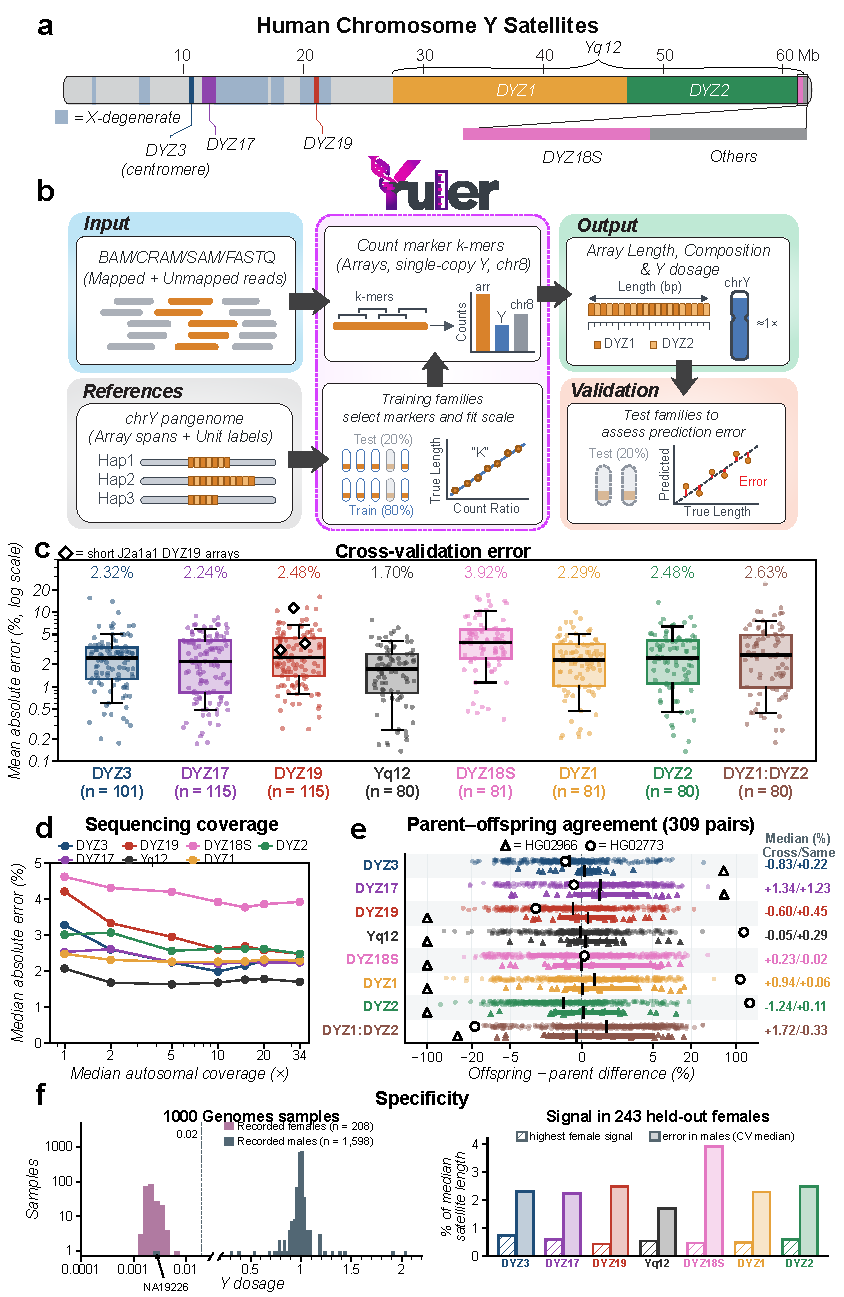
\includegraphics{figures/main/fig1_method.pdf}}
\caption{\textbf{Yruler measurement and validation.} \textbf{a}, Y satellite arrays and Yq12 components, with X-degenerate regions in blue. \textbf{b}, Workflow with family-grouped training and testing. The autosomal window is on chromosome 8. \textbf{c}, Absolute percentage errors for seven targets and the DYZ1:DYZ2 ratio. Points show each male's mean error across ten repeats of 5-fold cross-validation, and labels give pooled median errors. Diamonds: short J2a1a1 DYZ19 arrays. Logarithmic axis. \textbf{d}, Runtime and peak memory on 130 whole-genome CRAMs. In c--d, boxes show interquartile ranges, central lines medians and whiskers 10th--90th percentiles. \textbf{e}, Median errors after downsampling the test reads of the 130 cross-validation males (82 to 126 per target). \textbf{f}, Relative offspring--parent differences, $100(\mathrm{offspring}/\mathrm{parent}-1)$, in 309 pairs, with medians by batch contrast. Open triangles: HG02966. Open circles: HG02773. Scale linear within $\pm5\%$, logarithmic outside. Y dosage by sex and in read mixtures are in Extended Data Fig.~\ref{fig:no_y_cut}a,b.}\label{fig:method}
\end{figure}

\begin{figure}[tbp]
\centering
\makebox[\textwidth][c]{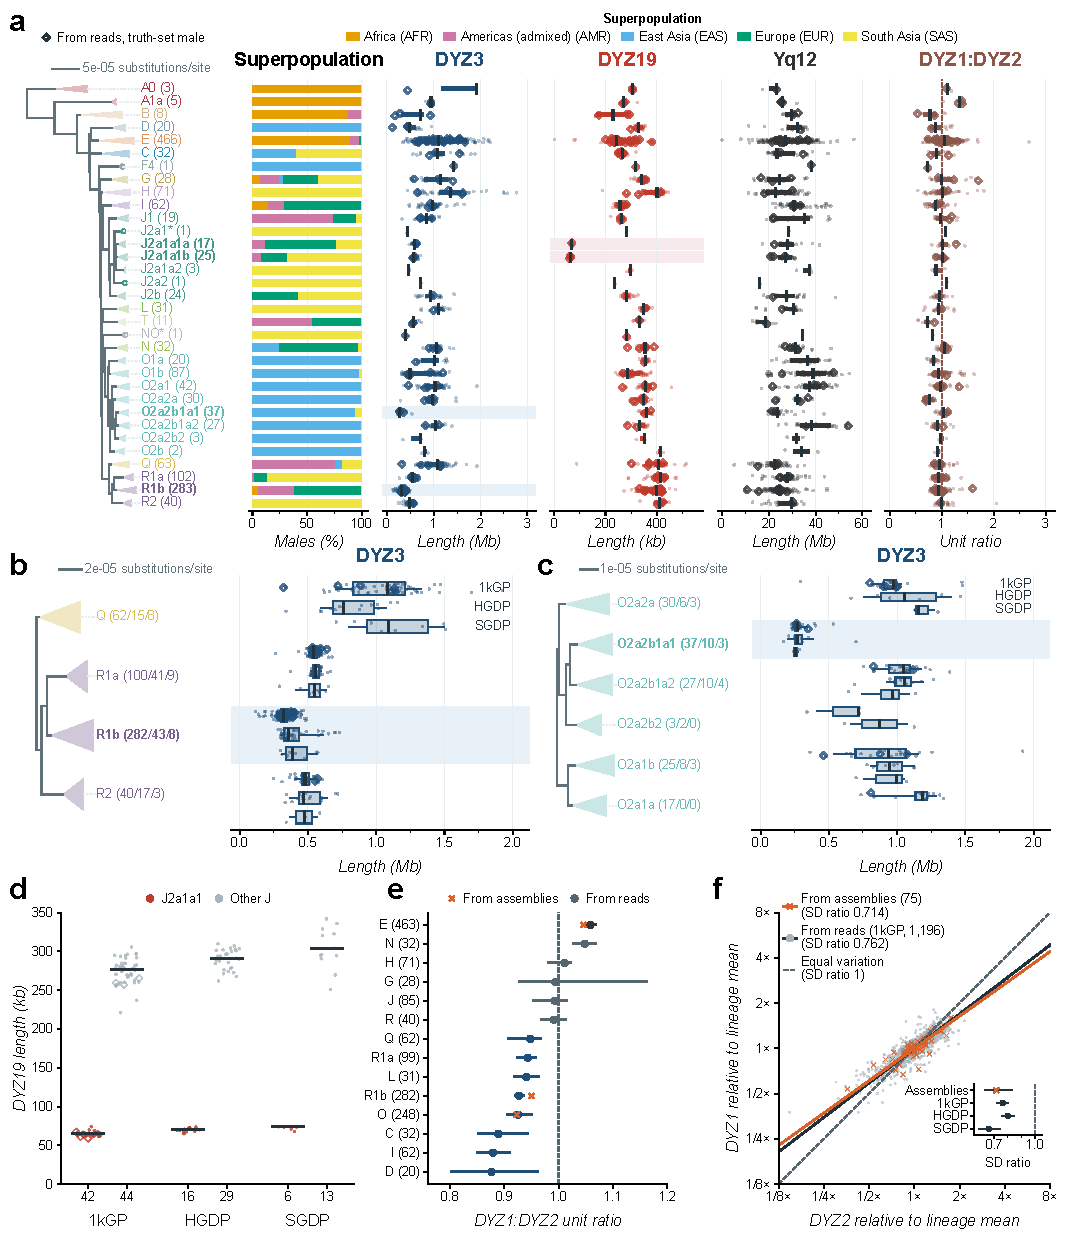
\includegraphics{figures/main/fig2_biology.pdf}}
\caption{\textbf{Y satellite variation across paternal lineages.} \textbf{a}, Single-nucleotide polymorphism (SNP) tree of 1,597 1000 Genomes Project (1kGP) males, with collapsed haplogroup clades, cohort-reported superpopulation proportions and satellite measurements. Counts in brackets give the males of each clade in the tree. Bars show interquartile ranges and ticks medians for clades with at least five males, over the 1,587 males of the population summaries, or 1,583 for Yq12 and the ratio. Shading highlights R1b and O2a2b1a1 in DYZ3, and J2a1a1 in DYZ19. \textbf{b}, DYZ3 in R1b and other lineages by cohort. \textbf{c}, DYZ3 in O2a clades, with cohorts ordered 1kGP, HGDP, SGDP. Boxes show interquartile ranges, central lines medians and whiskers 10th--90th percentiles. \textbf{d}, DYZ19 in J2a1a1 and other J lineages, excluding four Yp-depleted males from 1kGP. Fold annotations give ratios of group medians, and numbers indicate sample sizes. \textbf{e}, DYZ1:DYZ2 unit ratios from reads (dots, medians and 95\% intervals from resampling kinship components) and assemblies (crosses). Dashed line: equal numbers of units. \textbf{f}, DYZ1 and DYZ2 lengths divided by their lineage geometric means, on logarithmic axes, in 1,186 1kGP males without reference assemblies and 83 assemblies \cite{Hallast2026}. Lines have slopes SD(log DYZ1)/SD(log DYZ2), with SD the standard deviation, with 1 indicating equal variability. Inset: ratios for assemblies and the three cohorts (HGDP 386 males, SGDP 151), with 95\% bootstrap intervals. Open diamonds in a--d mark individuals with reference assemblies for that target. These estimates may be in-sample. Tests in b--d are two-sided Mann--Whitney tests and in f Pitman--Morgan tests, with P values in the Methods; 1kGP tests use one male per kinship component.}\label{fig:biology}
\end{figure}


\clearpage
\section*{Methods}\label{sec:methods}
\setcounter{secnumdepth}{0}
\renewcommand{\thetable}{M\arabic{table}}

\subsection{Reference arrays}\label{sec:m-truth}
\vsette{Reference arrays came from the 142-individual Y pangenome resource \cite{Hallast2026}, with HPRC release 2 replacements where the corresponding primary-resource array failed completeness criteria \cite{HPRCRelease2}. The inventory contained 129 DYZ3 spans (120 primary-resource and nine replacement arrays), 91 Yq12 regions (83 and eight), and 140 candidate spans each for DYZ19 and DYZ17. Eligibility was assessed separately for each target: an array had to lie on one contig, have at least 100 kb of flanking sequence on both sides and contain no assembly gap. We also excluded a target if the same overlapping 1 kb genomic bin contained an error flag from all four quality tracks: Flagger and NucFlag, each with HiFi and ONT reads. This bin rule records concordant local flags; it does not require the four flagged intervals to coincide base for base or certify every retained base as correct.}

\vsette{HG03098 failed the gap check for DYZ19. The four-track rule excluded the Yq12 and DYZ2 targets of HG01261; its DYZ1 and DYZ18S annotations remained eligible, and its regions stayed in marker selection (removing them would add 3,698 Yq12-class and 266 DYZ2 markers, remove none, and change Yq12 by a median of 0.0055\%, maximum 0.0267\%, in the 115 calibration males). The resulting reference panels contain 129 DYZ3, 90 Yq12, 91 DYZ1, 90 DYZ2, 91 DYZ18S, 139 DYZ19 and 140 DYZ17 targets. Matching short reads were available for 101, 80, 81, 80, 81, 115 and 115 individuals, respectively, in the reported cross-validation. The 21 held-out males were excluded from model choice and from these evaluated training panels (Accuracy evaluation, below).}


\subsection{Satellite annotation}\label{sec:m-units}
\vsette{Reference lengths follow the published Hallast annotation \cite{Hallast2026}. For Yq12, we used the HMMER motifs DYZ1\_Yq, DYZ2\_Con, DYZ18\_Yq, Yqhet\_3k1bp and Yqhet\_2k7bp and the script \texttt{filterYq12HMMER.py} of the repository \url{https://github.com/Markloftus/PanYChromosome} \cite{Hallast2026}, with the motifs of \url{https://github.com/core-unit-bioinformatics/project-chrom-y-extended} (commit 6da9f08). Class amounts are sums of end minus start over the retained blocks, rather than numbers of motif hits. This reproduces the published DYZ1 and DYZ2 amounts in Supplementary Table 26 of Hallast et al. \cite{Hallast2026} for all 84 comparable assemblies. Assemblies without a published annotation, including the HPRC replacements, were processed with the same motifs, nhmmer options and filters, using the published database size of 54.195246 Mb \cite{Hallast2026,Wheeler2013}. DYZ1 and DYZ2 targets are their respective block-length sums; DYZ18S is the sum of the DYZ18 and 3.1 kb block lengths. DYZ3 and the complete Yq12 region use the reference array coordinates. DYZ19 uses the main-array span returned by the script \texttt{filterDYZ19HMMER.py} of the same repository \cite{Hallast2026}.}

\vsette{DYZ17 was not included in that published annotation, so its reference lengths, and its CV errors, rest on our own annotation rather than an independent one. We constructed its profile from start-to-start repeat units in 140 assemblies, aligned them with MAFFT \cite{Katoh2013}, built an HMM with hmmbuild and emitted a 5,573 bp consensus with hmmemit \cite{Eddy2011}. We searched with the published DYZ1 nhmmer options \cite{Hallast2026}. The DYZ17 target is the outer-coordinate span of the longest run of hits separated by gaps of at most 10 kb; it is an array span rather than the sum of hit lengths.}

\vsette{Our separately constructed profile-HMM annotation of the same Yq12 arrays is retained to delimit the regions from which marker candidates are sampled. The distinction is intentional: reference amounts for fitting and scoring follow Hallast et al. \cite{Hallast2026}, whereas sampling regions for the Yq12-class markers follow our annotation. Selecting markers directly from the published blocks admitted copy-variable markers where motif boundaries differed. The comparison and the rule used to choose the sampling variant are disclosed under Accuracy evaluation. All calibration, inner model choice and scoring use the annotation lengths without any adjustment for marker-copy counts.}

\subsection{Markers from the Y pangenome}\label{sec:m-markers}
\vsette{Canonical 31-mers were counted in assembly regions with KMC 3.2.4 \cite{Kokot2017}. Candidate pools contain k-mers present in at least 15\% of the class assemblies and absent from the non-Y sequence of CHM13 \cite{Nurk2022} and all 71 selected HPRC release 2 haplotypes. Those haplotypes exclude study individuals and their recorded relatives. Within a training partition, a class marker must be present in at least a fraction $p$ of eligible class assemblies and occur outside the class on fewer than a fraction $o$ of the training Y assemblies; $o=0$ requires no such outside occurrence. The candidate grid is $p\in\{0.50,0.60,0.70,0.80,0.90,0.95\}$ and $o\in\{0,0.05,0.10,0.25\}$. DYZ18S sampling regions combine DYZ18 and the 3.1 kb repeat. The Yq12 residual helper samples the part of the Yq12 region outside the DYZ1 and DYZ2 sampling regions.}

\vsette{Each class's presence and outside thresholds are selected by five-fold cross-validation inside the outer training partition. Recorded families remain together. For every candidate rule, marker sets, the single-copy ruler and the scale are rebuilt from the inner training data and evaluated on the inner test data; the rule with the smallest pooled median absolute percentage error across the five inner folds is retained, then refitted on the complete outer training partition. Only the outer test errors enter the benchmark. A rule is eligible only when scored in every inner fold. We check that the 15\% candidate pool contains every marker an eligible training-fold rule can select, including after the inner split. The production model refits the same procedure on all eligible training individuals. Fixed development choices and use of outer CV to choose the sampling variant are disclosed separately under Accuracy evaluation.}

\vsette{All classes use the same ruler: X-degenerate Y k-mers present in at least 90\% of the training assemblies, with the non-Y filter also applied. The selection uses presence, not copy number: in 149 assemblies a median of 99.49\% of ruler keys occurred once on the Y (minimum 97.43\%), and keys with two or more copies carried 0.83\% of the ruler sum (maximum 4.75\% in NA21093). Removing the 605,313 keys with two or more copies in any assembly would change the ratio of the ruler sums in the 115 calibration males by a median of 0.04\% (maximum 2.02\%); this is an estimate without a new fit. Only DYZ2 has a minimum marker G+C content, 14 of 31 bases (45.2\%). This floor was chosen by a truth-free rule on ten PCR-free same-individual SGDP--1kGP pairs and retained because the DYZ2 marker sets are unchanged from the model on which that rule was applied; it is fixed during the nested CV, rather than selected by inner CV. No other reported class has a G+C floor. The sample-specific G+C correction curve is applied independently of this floor to every class.}

\vsette{Of the 28,650 DYZ18S markers, 10,384 (36.2\%) are also DYZ1 markers. The released marker counts are 6,183 for DYZ3, 504,611 for the Yq12 marker class, 201,987 for DYZ1, 30,176 for DYZ2, 28,650 for DYZ18S, 91,086 for DYZ19, 75,149 for DYZ17 and 45,561 for the unreported Yq12 residual helper, with 6,860,192 ruler markers. The reported Yq12 length is the component sum defined below, not the separately calibrated Yq12 marker-class estimate. A further 386,153 keys represent the autosomal dosage window at chr8:91--101 Mb, using its projections into 101 high-quality HPRC haplotypes. Masked superstrings \cite{Sladky2023} and zstd compression preserve marker membership while reducing file size. The released \texttt{model.tsv} gives scales and output expressions, and the released marker archive fixes the marker sets.}

\subsection{Read-based marker counting}\label{sec:m-counting}
Yruler reads BAM, CRAM, SAM, FASTQ and FASTA files through HTSlib \cite{Bonfield2021}, the text formats plain or gzip-compressed. With a BAM or CRAM index, it reads parallel genomic shards: whole-file shards are 10 Mb windows plus unmapped reads, and restricted-region mode uses merged BED intervals plus unmapped reads. Without an index, and for SAM, FASTQ and FASTA, it reads each file from start to end; a comma-separated list reads several files, such as the two FASTQ files of read pairs. Overlapping retrievals are deduplicated by their shard ownership so that an eligible record is counted once. Secondary and supplementary records are excluded. Primary records are retained without a mapping-quality threshold, and neither duplicate flags nor quality-check failure flags exclude reads from marker counting. Bases written as \texttt{=} cannot be read without the alignment, so Yruler stops without output on such files. Paired-end reads contribute as separate sequencing records, and every canonical 31-mer occurrence contributes to its marker count. Ambiguous bases interrupt k-mer generation. The current counting path does not apply a base-quality threshold.

An open-addressing hash table verifies marker membership after a Bloom filter, with thread-local caches reducing repeated lookups. A marker may contribute to multiple classes, as required when a component is also part of Yq12. \vsette{Class counts, the Y ruler and chr8-window counts are accumulated together; outputs include per-marker counts, class summaries, genomic-position summaries and normalized estimates; read sequences are written only on request.} SAM input is read sequentially and processed in parallel. The restricted-region BED is specific to the alignment pipeline and requires its own scale calibration.

\subsection{Length estimation}\label{sec:m-length}
\vsette{For individual $i$ and directly calibrated marker class $c$, let $C_{ik}$ be the count of marker $k$ and $g(k)$ its number of G or C bases. We estimate a relative depth curve $r_i(g)$ from single-copy Y markers. Counts above ten times the mean count plus ten are left out of the curve fit; the baseline is the mean of the remaining counts, and each G+C-bin mean uses the remaining counts of its markers. A supported bin requires at least 1,000 markers and 10,000 retained counts; an unsupported bin uses the nearest supported G+C bin. The same rule applies at every sequencing depth. Dividing bin means by the baseline gives $r_i(g)$. Let $f_i$ be the mean of $r_i(g(k))$ over the ruler markers, so that}

\vsette{\begin{equation}
 S^{\mathrm{GC}}_{ic}=f_i\sum_{k\in M_c}\frac{C_{ik}}{r_i(g(k))},
 \qquad S_{iY}=\sum_{k\in M_Y}C_{ik}.
\end{equation}}

\vsette{The curve requires at least 1,000,000 ruler counts and at least one supported bin. Without a usable curve, a sample above the no-Y dosage cut ($D_i>0.0067$) retains the ruler denominator and uses uncorrected sums, as in CV. At or below the cut, Yruler reports marker background at haploid autosomal depth instead of treating the small ruler count as an array-length denominator (Y dosage, below). Ruler and autosomal-window sums are not G+C-corrected. Thus, lack of a curve alone does not withhold an otherwise Y-positive estimate.}

\vsette{For a directly calibrated class the estimate and training scale are}

\vsette{\begin{equation}
 \widehat L_{ic}=K_c z_{ic},\qquad
 z_{ic}=\frac{S^{\mathrm{GC}}_{ic}}{S_{iY}},\qquad
 K_c=\frac{\sum_{i\in\mathcal T_c}L_{ic}}
 {\sum_{i\in\mathcal T_c}z_{ic}},
\end{equation}}

\vsette{where $\mathcal T_c$ contains training individuals with an eligible annotation length for class $c$. The scale relates marker abundance to that target; marker occurrences are not assumed to measure physical base coverage directly. Reference amounts are not changed according to the selected markers. For the residual helper, the training target is the reference Yq12 span minus the DYZ1 and DYZ2 block-length sums of Hallast et al. \cite{Hallast2026}. Its scale is fitted in the training partition in the same way as other classes. The reported total is}

\vsette{\begin{equation}
 \widehat L_{i,\mathrm{Yq12}}=
 \widehat L_{i,\mathrm{DYZ1}}+
 \widehat L_{i,\mathrm{DYZ2}}+
 \widehat L_{i,\mathrm{DYZ18S}}+
 \widehat L_{i,\mathrm{Yq12rest}}.
\end{equation}}

\vsette{The residual is the annotated Yq12 span minus its DYZ1, DYZ2 and DYZ18S units (other repeats and unannotated sequence) and has its own marker class and scale. On the same 80 males and folds, this sum gave Yq12 cross-validation errors equal to the sum of DYZ1, DYZ2 and a residual that contains DYZ18S (median 1.72\% for both; maximum 8.16\% and 8.04\%) and lower than the standalone Yq12 marker class (median 1.75\%, maximum 9.22\%). Inner selection, outer CV, lineage exclusion and held-out evaluation use the same output expression. The standalone Yq12 marker class is retained in the parameter file, but its own scale and marker sum are not the reported total. The released calibration is for Illumina whole-genome reads; other library types require their own evaluation.}

\subsection{Y dosage}\label{sec:m-dosage}
Y dosage is
\begin{equation}
 D_i=\frac{2}{s}\,\frac{S_{iY}/n_Y}{S_{iA}/n_A},
\end{equation}
where \vsette{$S_{iA}$ is the raw marker sum of the autosomal window at chr8:91--101 Mb, $n_Y$ and $n_A$ are the marker-set sizes and $s=0.9614$ is the median unscaled ratio in the 1kGP samples with dosage above half the cohort median (the same scale gives medians of 1.002 in HGDP and 1.025 in SGDP, so dosage thresholds apply to 1kGP-like libraries)}. Under balanced sequencing and one Y chromosome per diploid cell, $D_i$ is expected to be near one. \vsette{Copy-number changes of the window} and differential sequence representation can change this ratio. In a structurally altered Y chromosome, gains and losses of ruler-bearing regions can also change dosage; it cannot then be interpreted directly as the number of Y chromosomes or centromeres. An estimable positive length for all \vsette{seven} targets is required. \vsette{With fewer than 1,000,000 single-copy Y counts there is no G+C curve: above the no-Y cut ($D_i>0.0067$, the highest of 208 1kGP females) the estimate is the ratio to the ruler without G+C correction, as in cross-validation, and at or below the cut the output is background at haploid autosomal depth.} A uniform change in Y abundance cancels in the array-to-Y ratio, so dosage below 0.9 alone is retained as a descriptive flag. Arm imbalance is assessed separately using the chromosome-arm profiles below.


\vsette{Cohort X, PAR1 and PAR2 dosages use 31-mers of the high-quality HPRC haplotypes, counted in one pass: the mean key count is divided by the mean count of the chromosome 8 window and by its median in the reference males, so X 1 means one copy and PAR 1 means two copies (X + Y). The chrY profiles use CHM13v2 chrX 31-mers that occur on no autosome, on chrM or on chrY (one in 32 kept), counted in the reads that the CRAM file places on chrX, chrY or chromosome 2 or leaves unmapped, with the same denominator; PAR1, PAR2 and X-transposed profiles use 31-mers present on both chrX and chrY in those regions.} A sex-chromosome label gives the X and Y copies when both dosages are within 0.15 of a whole number and mosaic otherwise.

\subsection{Checks without assembly lengths and library metadata}\label{sec:m-truthfree}
The female background of each class is the estimate of a held-out female genome with the Y ruler replaced by its expected sum at the female haploid depth. Mixtures combine read pairs sampled from the alignment files of a male and a female at the Y fraction and its complement, so that mates stay together, and are compared with the whole genome of the same male. Read loss by G+C content was simulated on per-marker counts split by read G+C (reads re-counted with Yruler in nine G+C bins) by binomial thinning of each bin. Library type comes from CRAM read groups (HGDP), the SGDP sequencing panel and the project descriptions \cite{Bergstrom2020,Mallick2016,ByrskaBishop2022}; flowcells and project names come from the CRAM headers.

\subsection{Accuracy evaluation}\label{sec:m-benchmark}
Prediction accuracy was evaluated with ten repeats of random five-fold cross-validation, with \vsette{four folds used for training and one for testing}. Splits were randomized subject to keeping individuals with the same recorded pedigree FamilyID in the same fold; individuals absent from the pedigree were treated as separate groups. Among the \vsette{115} unique evaluated individuals, there were \vsette{114} such groups: only HG02666 and HG02668 shared a FamilyID (GB40). Their recorded test-fold assignments agreed in all ten repeats. In each repeat, group identifiers were randomly permuted and assigned cyclically to five folds; each fold served once as the test set. Thus, train/test proportions could vary slightly with group size and target-specific reference availability. Markers, the selection of their presence and outside thresholds and $K_c$ were fitted using only the outer training folds; the DYZ2 G+C floor, the reference-quality rule and the target definitions were fixed before cross-validation, and each individual's error was recorded in its outer test fold. Candidate k-mer pools were checked to contain every marker that could satisfy the training-fold selection rules, including those contributed by eligible reference assemblies without read data. \vsette{Three choices used results outside this scheme and are disclosed here. The final model was chosen between two marker-sampling variants by a rule written before their results, applied to the outer CV errors, so the reported CV is conditional on that choice: the variant that samples markers from the published blocks was kept unless its median absolute error was worse by more than 0.5 points, or its 90th percentile by more than 2 points, in at least one of Yq12, DYZ1, DYZ2 and DYZ18S. It was worse for DYZ18S (median 4.48\% against 3.93\%, 90th percentile 13.93\% against 10.42\%), so the variant that samples from our annotation was used. The DYZ2 G+C floor (14 of 31 bases) was chosen on the ten SGDP--1kGP PCR-free pairs after the CV of an earlier model had been seen; these pairs therefore are not independent validation of the floor. YqHet2.7 and DYZ18sub were dropped after their CV results (median errors 13.11\% and 5.63\%). The 21 held-out males were used in no choice. HG03248 has the most negative mean DYZ19 error of the panel ($-16.00\%$) and was retained.}

We additionally excluded each of 18 broad Y lineages in turn, removing its eligible references and any recorded family shared with test individuals from training. Markers, thresholds and calibration were refitted on the remaining references. Each evaluated individual therefore has one excluded-lineage prediction per target, rather than ten repeated CV predictions (Extended Data Fig.~\ref{fig:lineage-validation}). The same target-specific individuals were evaluated in both analyses.

For sequencing-depth sensitivity, test reads were thinned to \vsette{30, 25, 20, 15, 10, 5, 2 and 1$\times$ of base coverage}; training reads remained at full depth. All ten repeats and five folds were retained at every \vsette{level}, with the same test assignments as full-depth CV. Each \vsette{level} contains \vsette{6,530} predictions across the \vsette{seven} targets. All \vsette{6,530} full-depth predictions match the main CV in sample, repeat, fold and error. Coverage was measured from chromosome 2 \vsette{31-mer} counts in each thinned run\vsette{ and converted to base coverage (150/120)}; group coordinates are medians across the \vsette{115} unique evaluated individuals, each counted once. The seven \vsette{displayed} median coverages \vsette{are 1.0, 2.0, 5.0, 10.0, 15.0, 20.0 and 34.1$\times$. HG02953, below 30$\times$ at full depth, keeps its full-depth counts at the 30$\times$ level. The 30 and 25$\times$ levels are in the results table and are not displayed.}

The DYZ1:DYZ2 length ratio is a derived, dimensionless measurement rather than an additional satellite class. Its validation pairs the two component predictions for the same individual, repeat and test fold; fold assignments were checked to match. Ratio error is $100| (\widehat L_{\mathrm{DYZ1}}/\widehat L_{\mathrm{DYZ2}})/(L_{\mathrm{DYZ1}}/L_{\mathrm{DYZ2}})-1|$, calculated before summarizing. The paired set contains the \vsette{80} individuals with both references, with \vsette{800} full-depth predictions and ten repeats at each reduced coverage. Each excluded-lineage ratio likewise uses the two component predictions from the same held-out lineage. The ratio has no separately fitted calibration or marker set.

\begin{table}[tbp]
\caption{Cross-validation and excluded-lineage errors for \vsette{seven} satellite targets and their derived DYZ1:DYZ2 ratio. Values are absolute percentage errors. Mean, median, P90 and maximum pool the out-of-fold predictions. Maximum is a single prediction, made with the rule selected in that fold, not an individual mean. CV $n$ counts unique evaluated individuals. Lineage-out is the pooled median of one prediction per individual after excluding its lineage. Eligible-reference counts are in Table~\ref{tab:reference-lineages}.}\label{tab:accuracy}
\centering\small
\begin{tabular}{lrrrrrr}
\toprule
Target & CV $n$ & Mean & Median & P90 & Maximum & Lineage-out \\
\midrule
DYZ3 & \vsette{101} & \vsette{2.76} & \vsette{2.32} & \vsette{5.18} & \vsette{15.92} & \vsette{2.39} \\
Yq12 & \vsette{80} & \vsette{2.02} & \vsette{1.72} & \vsette{4.23} & \vsette{8.16} & \vsette{1.89} \\
DYZ1 & \vsette{81} & \vsette{2.66} & \vsette{2.29} & \vsette{5.40} & \vsette{10.48} & \vsette{2.30} \\
DYZ2 & \vsette{80} & \vsette{2.97} & \vsette{2.50} & \vsette{6.39} & \vsette{13.65} & \vsette{2.33} \\
DYZ18S & \vsette{81} & \vsette{4.87} & \vsette{3.92} & \vsette{10.42} & \vsette{17.63} & \vsette{4.09} \\
DYZ19 & \vsette{115} & \vsette{3.31} & \vsette{2.48} & \vsette{6.65} & \vsette{25.47} & \vsette{2.63} \\
DYZ17 & \vsette{115} & \vsette{2.77} & \vsette{2.24} & \vsette{5.92} & \vsette{12.19} & \vsette{2.40} \\
DYZ1:DYZ2 & \vsette{80} & \vsette{3.63} & \vsette{2.61} & \vsette{7.68} & \vsette{24.40} & \vsette{2.28} \\
\botrule
\end{tabular}
\end{table}

\subsection{Comparison with depth-based estimates}\label{sec:m-sanroman}
Published DYZ1 coverage values \cite{SanRoman2024} come from low-coverage Phase 3 reads. \vsette{On the same Phase 3 runs of 30 males with assembled arrays, whose libraries were PCR-amplified, the coefficient of variation of assembled length divided by estimate, which does not depend on any scale factor, was 27.52\% for the published values and 16.24\% for Yruler for Yq12, and 25.15\% and 23.57\% for DYZ1; Spearman correlations with assembled length were 0.400 and 0.800 for Yq12 and 0.475 and 0.539 for DYZ1. Each method scaled to base pairs with its own factor fitted on these males gave errors of 24.96\% and 20.15\% for the published values and 10.93\% and 20.52\% for Yruler. These errors come mainly from the libraries, because PCR-free reads thinned to 1$\times$ gave 2.06\% and 2.48\%.}

\subsection{Nanopore reads (preliminary)}\label{sec:m-ont}
Yruler is calibrated and evaluated on Illumina whole-genome reads. \provisional{The same procedure applied to nanopore reads learns markers, thresholds and scale factors from those reads within the training folds. In ten repeats of five-fold cross-validation on the 84 HPRC males with R10.4.1 reads (dorado super-accuracy base calls) \cite{HPRCRelease2} and assembled arrays, median absolute errors were 6.74\% for DYZ3 (78 males), 5.99\% for Yq12 (62), 4.31\% for DYZ1 (63), 8.95\% for DYZ2 (62), 9.71\% for DYZ18S (63), 7.05\% for DYZ19 (84) and 7.47\% for DYZ17 (84), 1.9 to 3.6 times those of short reads, with 90th percentiles of 12.76--23.79\% and maxima of 22.44--40.58\% (Table~\ref{tab:ont}). These nanopore values are preliminary and will be updated with the released marker set.} Nanopore estimates are therefore suited to checking unusual short-read results, as for HG01967, HG02895 and HG03685, rather than to fine comparisons between males. Corrected nanopore reads and PacBio HiFi reads remain to be tested.

\begin{table}[tbp]
\caption{Cross-validation errors of nanopore estimates (preliminary). Absolute percentage errors in ten repeats of five-fold cross-validation on HPRC R10.4.1 reads, with markers, thresholds and scale factors learned from nanopore reads in the training folds; short-read medians from Table~\ref{tab:accuracy}.}\label{tab:ont}
\centering\small
\begin{tabular}{lrrrrrr}
\toprule
Target & Males & Mean & Median & P90 & Max & Short-read median \\
\midrule
DYZ3 & \provisional{78} & \provisional{7.85} & \provisional{6.74} & \provisional{14.67} & \provisional{40.58} & 2.32 \\
Yq12 & \provisional{62} & \provisional{6.97} & \provisional{5.99} & \provisional{16.30} & \provisional{25.95} & 1.72 \\
DYZ1 & \provisional{63} & \provisional{5.73} & \provisional{4.31} & \provisional{12.76} & \provisional{22.44} & 2.29 \\
DYZ2 & \provisional{62} & \provisional{11.36} & \provisional{8.95} & \provisional{23.79} & \provisional{36.41} & 2.50 \\
DYZ18S & \provisional{63} & \provisional{10.94} & \provisional{9.71} & \provisional{22.32} & \provisional{36.85} & 3.92 \\
DYZ19 & \provisional{84} & \provisional{8.22} & \provisional{7.05} & \provisional{17.22} & \provisional{29.71} & 2.48 \\
DYZ17 & \provisional{84} & \provisional{8.49} & \provisional{7.47} & \provisional{17.54} & \provisional{25.80} & 2.24 \\
\botrule
\end{tabular}
\end{table}

\subsection{Pedigrees and sequencing batches}\label{sec:m-pedigree}
Parent--offspring pairs are XY pairs that share one Y transmission. These relationships were taken from the recorded 1000 Genomes parents; CEPH 1463 development comparisons used the published pedigree \cite{Porubsky2025}. Intersecting documented pairs with the 1,597 male-labelled samples with estimates gave 309 parent--offspring pairs: 282 have parents in the original 2,504-sample batch and offspring in the additional 698-sample batch, 25 have both in the additional batch, and two have the opposite cross-batch direction (NA07034--NA07048 and NA12056--NA10851). All 309 pairs are retained in the absolute-length panels and overall summaries. The main signed-difference panels summarize the 282 original-parent/additional-offspring pairs and the 25 same-batch pairs; the two reverse-direction pairs are shown separately in the absolute-length panels. Seventy-eight pairs involve at least one male with a reference assembly, 68 of them a calibration male; the other 231 involve two males without one. Arm-flagged pairs remain visible for structural follow-up.

\subsection{Population descriptors and reference-panel representation}\label{sec:m-descriptors}
Y haplogroups describe branches of the paternal genealogy inferred from Y-linked variants. They provide the grouping relevant to these Y satellite measurements and do not describe an individual's genome-wide ancestry, ethnicity or identity. Collapsing branches for display does not imply uniform satellite lengths within a lineage. The 1kGP population and superpopulation labels are retained as source metadata for sample accounting; they were not used to select markers, fit calibration scales or assign random cross-validation folds. Geographic coordinates describe locations reported by the source cohorts. We did not estimate genome-wide ancestry from Y haplogroups or geographic labels.

\subsection{Population summaries and composition}\label{sec:m-population}
We analysed 1,639 1000 Genomes samples using the model calibrated on the 115 males with reads and reference arrays. Of 1,598 male samples, 1,597 had estimable positive lengths for all \vsette{seven} targets; \vsette{sixteen} had dosage below 0.9, including \vsette{fourteen} with concordantly reduced arm signal, HG00185 with Yq loss \vsette{and HG03006 with Yp depletion}. Forty-one samples are female. The male without an estimate, NA19226, has one X and no Y signal; both pedigrees and KING (kinship 0.249 and 0.247, IBS0 0.00012 and 0.00008) make this sample the parent of NA19224, an XY offspring, so the Y was lost in its sample.

One hundred and thirty-six estimated individuals have reference assemblies: 115 entered the calibration, so their estimates can be in-sample, and 21 were held out. The other 1,461 have no reference assembly. The analysed subset covers all 26 1kGP populations; cohort labels and geographic coverage remain uneven. Four arm-imbalanced profiles (HG00185, HG01967, HG02966 and NA20806) and six Yp-depleted profiles (HG01982, HG01984, HG03006, HG03008, HG03976 and HG03998) remain visible but are excluded from population medians, interquartile ranges, correlations and relatedness sensitivity summaries, leaving 1,587 individuals. \vsette{Four males with a PAR2 gain (HG02773, HG02895, HG03685 and NA11930) leave the Yq12, DYZ1, DYZ2 and ratio summaries only, leaving 1,583 individuals for these.} \vsette{Fourteen} samples with concordantly reduced arm signal and available estimates are retained, including HG00246 and NA20754, whose arm ratios are both below 0.5. A separate sensitivity subset restores the earlier dosage threshold of 0.9. Screening states are not independently confirmed karyotypes. Reference cross-validation retains every individual and applies no dosage-based exclusion. Pedigree displays retain flagged pairs for follow-up.

Lengths are summarized by broad lineage and finer clades, retaining all represented groups in supplementary plots. R1b is compared with other chromosomes to assess a previously reported DYZ3 association \cite{Hallast2023}. Family and kinship-component sensitivity results accompany all-sample and outside-reference-panel summaries (Table~\ref{tab:relatedness}).

\vsette{Read-based composition uses the calibrated DYZ1 and DYZ2 amounts and their dimensionless length ratio. Both share the Y-ruler denominator. The reported Yq12 total is their sum with DYZ18S and a separately calibrated residual; it is therefore not statistically independent of its components. Repeat-unit ratios use the unit convention of Hallast et al. \cite{Hallast2026} rather than assuming that base-pair ratios count units.}

\vsette{The assembly-composition supplement uses 91 complete Yq12 references (83 primary-resource and eight HPRC release 2), with the published annotation \cite{Hallast2026} or the same procedure on replacements. Annotation records match the exact assembly and contig in the reference manifest. DYZ1, DYZ2, the sum of DYZ18, 3.1 kb and 2.7 kb block lengths, and residual unannotated bases partition each reference-coordinate span; this identity was checked per array.} Individuals follow clade order and are sorted by DYZ1 fraction within clades; seven references without matching lineage metadata remain in the supplement. The length--fraction plot is descriptive and its axes share the annotated span. The unresolved NO [K2a] call of HG03742 is displayed separately as NO in broad-lineage plots and NO* in the tree; its source annotation is retained.

\subsection{Chromosome-arm profiles and sequencing-run consistency}\label{sec:m-y-arms}
Arm-level quality control covered all 1,639 processed samples. Y ruler marker counts were summed separately over Yp (X-degenerate blocks XDR1--2, 850,505 markers) and proximal Yq (XDR3--8, 6,000,853 markers), each marker taking the block it occupies in at least 90\% of the assemblies that carry it, and divided by \vsette{the counts of the chromosome 8 window}. Each arm ratio was scaled to its median across samples with both raw ratios above half their initial cohort medians. These proximal-Yq markers do not measure the distal Yq12 satellite block. \vsette{Doses of the eight blocks also flag changes that the arm rule misses: among 1,565 males with a normal state, the median block dose differed from the key-weighted mean by more than 2\% in 12 males. The largest were NA20801, with XDR3 at 0.697, whose lengths are inflated by a predicted 7.95\%, and NA20809, with XDR7 at 1.344, whose lengths are deflated by a predicted 4.62\%; NA20809 is a calibration male with a median Yq12 error of $-5.12\%$, and $-0.50\%$ after this correction.} \vsette{PAR2 keys had a median of 0.996 copies on 117 Y-bearing and 0.998 on 348 other HPRC haplotypes, so one more whole copy predicts a dose of 1.49 from the median of normal males (0.9946); the four males with a PAR2 gain lay at 1.44--1.47, and a copy covering 90\% of PAR2 cannot be excluded. Independent libraries confirm the gains in the sample: NA11930 had PAR2 doses of 1.502, 1.425 and 1.510 in Aviti, NovaSeq and low-pass libraries, with Yq12 of 42.65, 43.85 and 56.54 Mb (the low-pass library read the control NA12342 6.0\% higher than its 1kGP library, 26.65 against 25.15 Mb); HG02895 had 1.453 and 1.468 in two ONT runs, HG03685 1.578 in ONT reads \cite{Gustafson2024} and HG02773 1.504 in a Polaris library, with Yq12 of 51.16 Mb (56.35 Mb in its 1kGP library). Doses were 0.964 in ONT reads and 1.004 in a Polaris library of the parent HG02771, whose Polaris Yq12 was 24.29 Mb (24.28 Mb in 1kGP), 1.019 in a control library and 0.948--1.137 in five ONT controls. In the hifiasm assembly of the HG03685 ONT reads \cite{Gustafson2024}, a 91.9 Mb contig carries PAR2 and 5.11 Mb of Yq12 joined to 89.3 Mb that align to CHM13 chromosome 15 from 5.98 Mb on the short arm. Aligned with minimap2 2.31 to the whole diploid assembly, 13 ONT reads of 17.0--61.4 kb crossed the junction in one alignment each, with 5.2--45.3 kb on either side, MAPQ 25--44 and 88.7--99.9\% of each read aligned; the extra PAR2 copy of HG03685 therefore sits with Yq12 on the short arm of chromosome 15, the configuration of a Yqh--acrocentric translocation \cite{Ng2006}. HG01589, HG03809 and HG04149 had PAR2 doses of 0.51--0.62 with normal PAR1, which suggests PAR2 losses that the screening rule does not flag.} \vsette{HG01882, HG02058 and NA11992 have Y dosage of 1.18--1.24, below the cut of 1.25, and remain in the normal state.}

The priority-ordered screening rule assigned negligible Y signal when whole-Y dosage was at most \vsette{0.0067}, the highest value in \vsette{208 1kGP} female genomes; Yp depletion when Yp was below 0.5 and Yq within 0.1 of one; Yq loss when Yp was within 0.1 of one and Yq more than 0.1 below Yp; arm imbalance when the absolute Yp--Yq difference exceeded 0.1\vsette{; and PAR2 gain when the PAR2 dose was at least 1.25 with PAR1 within 0.1 of one}. Among remaining samples, whole-Y dosage of at least 1.75, 1.25--1.75 or below 0.9 flagged Y gain, intermediate gain or low dosage, respectively. The remaining samples had no flag. The corresponding labels (\texttt{no\_Y}, \texttt{yp\_deletion}, \texttt{yq\_loss}, \texttt{partial}, \vsette{\texttt{par2\_gain}}, \texttt{Y\_gain}, \texttt{mosaic\_gain}, \texttt{mosaic\_loss} and \texttt{normal}) are screening categories, not confirmed karyotypes, deletion boundaries or mosaic fractions. Counts were 42 (41 females and NA19226), 6, 1, 3, \vsette{4}, 2, \vsette{2}, \vsette{14} and \vsette{1,565}, respectively. Y dosage is measured against chromosome \vsette{8}, so it does not name a karyotype: a separate column combines the X and Y dosages and gives XY (\vsette{1,576}), XX (40 of the 41 females), XXY (1), XYY (2), X (1) or, when either dosage is more than 0.15 from a whole number, mosaic (\vsette{19: 18} males, including the samples with intermediate Y dosage, and one female, HG00176, with X dosage \vsette{1.787}).

Six samples showed Yp ratios of \vsette{0.263--0.282} with proximal-Yq ratios of \vsette{0.986--1.043} (Table~\ref{tab:y-arm-flags}). They include parent--offspring pairs HG01982--HG01984 and HG03006--HG03008, consistent with inherited Yp variation. Recurrent multigene Yp deletions involving TSPY have been described \cite{Jobling2007}; sequence confirmation is needed to identify the specific deletion. \vsette{Yp holds 12.4\% of the ruler markers (850,505 of 6,860,192). Under stable proximal-Yq dosage, the ratio of Yq to whole-ruler dose predicts satellite-length inflation of 10.10--10.24\% in these six.} We excluded the uncorrected estimates; a Yq-only denominator requires separate calibration.

Three further samples had Yp/Yq imbalance (HG01967, HG02966 and NA20806) and one had Yq loss with an intact Yp (HG00185). Together with the six Yp-depleted samples, they are retained in displays and excluded from population summaries. \vsette{Fourteen} samples with concordantly reduced Yp and Yq signal and estimable lengths are included despite dosage below 0.9; the lowest are HG00246 and NA20754 (Y dosage \vsette{0.3190} and \vsette{0.3995}). A uniform multiplicative reduction in Y abundance cancels between the array and single-copy Y signals, whereas loss or gain of selected ruler regions need not cancel. This algebraic distinction motivates the inclusion rule; it does not establish the biological cause of low signal or identical measurement uncertainty at every Y dosage.

For the HG02965--HG02966 pair, reads were partitioned by flowcell using the CRAM read-group metadata and processed separately (Table~\ref{tab:y-flowcells}). Each sample has one recorded library spanning three flowcells, with four read groups per flowcell. Relative to the same individual's whole-library result, the offspring's Yp signal ranged from \vsette{0.994} to \vsette{1.013}, proximal-Yq signal from \vsette{0.993} to \vsette{1.003}, DYZ3 from 0.995 to \vsette{1.008} and the near-absent Yq12 signal from \vsette{0.962} to \vsette{1.019}. The near-absent DYZ19 signal varied more (\vsette{0.831--1.226}). The whole-library arm ratios were 1.910 for Yp and 1.082 for proximal Yq in the offspring. Thus, Yp excess and distal satellite depletion recur across sequencing runs. This argues against a flowcell-specific anomaly; shared library preparation and cell-line history remain possible sources. These are technical partitions of one library, not independent DNA preparations or independent validation of chromosome structure.

Nanopore sequencing of HG01967 (ENA ERR15140186, downloaded with checksum verification) also showed increased Y signal and reduced Yq12 abundance: dosage was \vsette{1.358} and the raw Yq12-to-ruler count ratio was \vsette{0.711}. The corresponding short-read quantities were \vsette{1.314 and 0.565, against a ratio of 2.916 in HG02965}. Agreement in direction across platforms supports the unusual profile. The marker-count ratios are not independently calibrated long-read array lengths, and these data do not establish rearrangement boundaries.

Profiles along CHM13v2 chrY place these signals (Supplementary Fig.~\ref{fig:chrY-unusual}). Each 100 kb window shows the median dose of the 31-mers of CHM13v2 chrY that occur on no other CHM13 sequence (14,401,261 k-mers at 48,425,773 positions), counted in the reads that carry a yruler marker and divided by \vsette{the count of the chromosome 8 window} and by the median of 100 XY males with Y state normal; each of the 625 windows has at least 50 k-mer positions in every sample. In HG02966, Yp11.2 is at 1.94 copies and Yq11.221 at 1.80, the windows \vsette{from 11.0} to 17.0 Mb are at \vsette{1.80--1.98}, the windows from 17.1 to 17.3 Mb are at 0.99 and 1.00, and every band from Yq11.222 through Yq12 is at 0. The windows at one copy hold the two arms of palindrome P6 (chrY:17,066,095--17,176,113 and 17,222,323--17,332,346) \cite{Rhie2023}, which share their 31-mers: a normal Y carries both arms and HG02966 carries two copies of one arm, the configuration expected for an isodicentric Y formed by recombination between palindrome arms \cite{Lange2009}. Its parent HG02965 shows no change (Yp11.2 \vsette{1.00}, Yq11.222 \vsette{0.98}). The centromere value of HG02966 (\vsette{2.13}, reference median 1.01) also reflects the size of its DYZ3 array, not only its copy number. HG01967 shows a similar pattern at lower amplitude: 1.61 in Yp11.2, 1.69 in Yq11.221, 0.31 in Yq11.223 and 0.27 in Yq12, consistent with 69\% of cells carrying such a chromosome (1 + 0.69 copies before the break, 1 $-$ 0.69 after it). Its transition lies in Yq11.222 and has two steps: windows up to 18.3 Mb are at 1.69--1.72, windows from 18.4 to 19.3 Mb at 0.81--0.99 and windows from 19.4 Mb at \vsette{0.23--0.55}. \vsette{In HG02773 and NA11930 the Yq12 windows are at 2.05 and 1.69, against 0.91 in the parent HG02771 and 0.83 in the offspring NA10845, while Yp11.2 (1.03 and 1.04) and Yq11.221 (0.98 and 0.99) are normal: the gain is limited to Yq12 and PAR2.} In \vsette{16} parent--offspring pairs with an unusual member (Supplementary Fig.~\ref{fig:chrY-pairs}), Yp depletion (two pairs), a long DYZ18S array and a short DYZ19 array were shared by parent and offspring, whereas mosaic gains and losses, the Y gain of HG03456, the XXY state of HG01683, the HG02966 rearrangement\vsette{, the PAR2 gain of HG02773 and of NA11930} and the Y loss of NA19226 were each seen in one generation. These doses do not distinguish germline changes from changes that arose in the cell lines.

\begin{table}[p]
\caption{Samples with arm-imbalanced or Yp-depleted marker profiles. Arm ratios are cohort-normalized; whole-Y dosage comes from the population estimate table. All ten samples are excluded from population summaries. These profiles require structural follow-up.}\label{tab:y-arm-flags}
\centering\small
\begin{tabular}{llrrr}
\toprule
Sample & Profile & Y dosage & Yp & Proximal Yq \\
\midrule
HG00185 & Yq loss & \vsette{0.787} & \vsette{1.013} & \vsette{0.755} \\
HG01967 & Yp/Yq imbalance & \vsette{1.315} & \vsette{1.684} & \vsette{1.262} \\
HG01982 & Yp depletion & \vsette{0.904} & \vsette{0.263} & \vsette{0.997} \\
HG01984 & Yp depletion & \vsette{0.906} & \vsette{0.268} & \vsette{0.998} \\
HG02966 & Yp/Yq imbalance & \vsette{1.186} & \vsette{1.910} & \vsette{1.082} \\
HG03006 & Yp depletion & \vsette{0.895} & \vsette{0.269} & \vsette{0.986} \\
HG03008 & Yp depletion & \vsette{0.906} & \vsette{0.270} & \vsette{0.998} \\
HG03976 & Yp depletion & \vsette{0.906} & \vsette{0.272} & \vsette{0.998} \\
HG03998 & Yp depletion & \vsette{0.947} & \vsette{0.282} & \vsette{1.043} \\
NA20806 & Yp/Yq imbalance & \vsette{1.015} & \vsette{1.161} & \vsette{0.994} \\
\botrule
\end{tabular}
\end{table}

\begin{table}[p]
\caption{Technical consistency across flowcells for parent HG02965 and offspring HG02966. Each sample has one recorded library. Depth is the mean count of the chromosome \vsette{8} window. DYZ3, Yq12 and DYZ19 columns give ratios to the same sample's whole-library measurement; the offspring's near-absent satellite signals must not be interpreted as normal absolute lengths.}\label{tab:y-flowcells}
\centering\scriptsize
\begin{tabular}{llrrrrr}
\toprule
Sample & Flowcell & Depth & Y dosage & DYZ3 & Yq12 & DYZ19 \\
\midrule
HG02966 & HV3CYDSXX & \vsette{8.19} & \vsette{1.186} & \vsette{0.995} & \vsette{1.016} & \vsette{0.887} \\
HG02966 & HV3GMDSXX & \vsette{8.48} & \vsette{1.182} & \vsette{0.995} & \vsette{0.962} & \vsette{0.831} \\
HG02966 & HV3HYDSXX & \vsette{10.47} & \vsette{1.187} & \vsette{1.008} & \vsette{1.019} & \vsette{1.226} \\
HG02965 & HTGLNDSXX & \vsette{10.10} & \vsette{0.995} & \vsette{1.010} & \vsette{1.013} & \vsette{0.997} \\
HG02965 & HV3CGDSXX & \vsette{9.30} & \vsette{0.997} & \vsette{0.996} & \vsette{0.993} & \vsette{0.993} \\
HG02965 & HV3KJDSXX & \vsette{9.41} & \vsette{0.995} & \vsette{0.993} & \vsette{0.993} & \vsette{1.011} \\
\botrule
\end{tabular}
\end{table}


\subsection{Geographic metadata and the haplogroup display}\label{sec:m-geography}
Geographic metadata come from the IGSR population table archived in the kgp package and public SGDP metadata \cite{Bergstrom2020,Mallick2016}. The map combines the 1,597 analysed 1kGP males with public manifests of 552 HGDP and 175 retained SGDP samples. The main length analyses use the 1kGP males; 518 PCR-free HGDP and SGDP individuals replicate the DYZ19, DYZ3 and DYZ1:DYZ2 results. Coordinates describe reported population locations, not individual residences, birthplaces or ancestral origins. The Mala population, absent from the archived IGSR table, uses the public SGDP coordinates.

Pie sectors use the source table's HaploGrouper ISOGG 2019 deCODE calls for 1kGP and published calls from Hallast et al. Supplementary Table 2 \cite{Hallast2021} for HGDP and SGDP. Missing published assignments were supplemented with HaploGrouper ISOGG 2019 calls from chrY genotypes for 21 individuals (17 HGDP and four SGDP). Joins use exact identifiers or documented aliases and never infer lineage from population membership. Seven SGDP records reported as female were excluded from the paternal-lineage map. This includes Peru60, whose Y dosage was 0.0053; NOR111, of unspecified reported sex and Y dosage 0.0044, was also excluded because its chrY calls showed no Y signal. These eight exclusions do not change the 1kGP length analyses. Before deduplication, 551 HGDP and 173 retained SGDP records have assignments. Calls agree for shared individuals with multiple assignments; a missing published call can be filled from a matched 1kGP record. Only HGDP00119 and SGDP\_HGDP00725 remain unassigned in the combined map, pending chrY genotypes. Grey sectors and the legend identify these two individuals.

\vsette{Figure~\ref{fig:biology}a uses a maximum-likelihood tree rather than a haplogroup classification hierarchy, built with the procedure of Hallast et al. \cite{Hallast2026}. Calls came from BCFtools 1.16 (\texttt{mpileup -q20 -Q20 -a AD,DP}, \texttt{call -m --ploidy 1}, \texttt{filter --SnpGap 5}, indels removed) inside the mask of the Y regions accessible to short reads \cite{Poznik2013}. A call was set to missing when its depth was below 3 or the called allele had less than 85\% of the reads, and VCFtools 0.1.16 kept sites with at most 5\% missing calls. The alignment holds every callable position (10,416,430 positions, 80,845 polymorphic, 243,864 distinct site patterns) in 1,597 males. RAxML 8.2.10 ran one maximum-likelihood search with GTRGAMMA, and 100 rapid bootstrap replicates gave branch support: median 100 over 1,594 internal branches, at least 95 for 65.9\% of them and at least 70 for 75.6\%. The splits of A0 from the other males, of E, J, R1b, J2a1a1a, J2a1a1b, O2a2b1a1, O2a2b1a2 and of the E1a2a1b2 pair had support 100, and the J2a1a1 clade 97. The root lies at the midpoint of the edge between the three A0 males (HG01890, HG02982 and HG02984) and the other 1,594. Branch lengths are substitutions per site, not dates.}

We prune this tree to the 1,597 analysed males, adding branch lengths when suppressing unary nodes. Homogeneous clades are collapsed into triangles that preserve their maximum descendant branch-length extent. The 29 displayed groups split O1a, O1b, O2a and O2b and retain J2a1a1a and J2a1a1b separately; all displayed rows are monophyletic at this resolution. J2a1* and NO* denote unresolved source assignments. No topology or sample order is chosen using satellite lengths. Extended Data Fig.~\ref{fig:j-dyz19} retains all 90 J tips; the 42 J2a1a1 individuals form a clade, with J2a1a2 outside it. The display is descriptive and does not estimate the number or timing of satellite-state transitions.

\subsection{Software performance}\label{sec:m-performance}
Whole-file and restricted-region runs were compared using the same input individuals and development marker set. Restricted-region windows were selected on 30 individuals and assessed on a separate 100. For each class, capture stability was summarized by the maximum minus minimum of the ratio of Y-normalized marker abundances from BED and whole-file counts, with a development acceptance threshold of 0.5 percentage points. A constant ratio offset is absorbed by a mode-specific scale and is distinct from variation in that ratio between individuals. Wall time and peak resident memory were measured separately from data transfer. Implementation changes were accepted only when marker counts and class summaries agreed; marker-read records were compared without assuming a stable output order under parallel reading.



\begingroup
\renewcommand{\figurename}{Extended Data Fig.}\renewcommand{\thefigure}{1}
\begin{figure}[tbp]
\centering
\makebox[\textwidth][c]{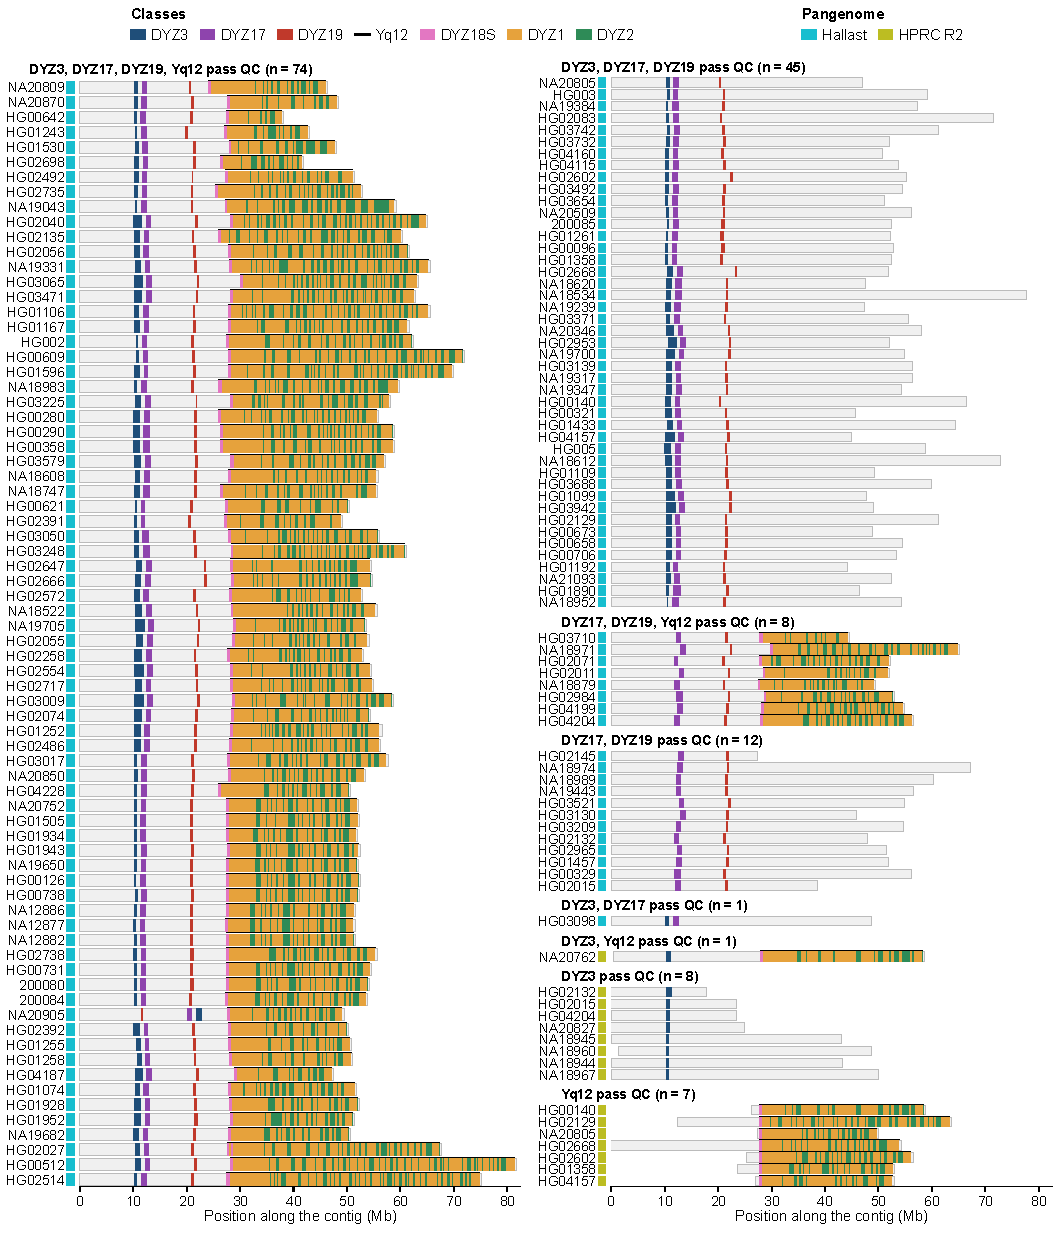
\includegraphics{figures/ed/ed1_array_structure.pdf}}
\caption{\textbf{Satellite arrays of the reference chrY assemblies.} One row per assembly (156), grouped by the arrays that pass quality control and serve for marker selection and training (DYZ3 129, DYZ17 140, DYZ19 139, Yq12 90). Colours mark the DYZ3, DYZ17 and DYZ19 arrays, and the DYZ1, DYZ2 and DYZ18S (DYZ18 and 3.1-kb repeats) clusters of at least 10 kb inside Yq12. The black line marks Yq12. The square left of each row marks the source: Hallast 2026 assemblies \citep{Hallast2026} as chromosome-scale contigs in the T2T orientation, and HPRC release 2 (HPRC R2) contigs \citep{Lucas2026}, placed at the median position of their first array. Rows in each group are ordered by average-linkage clustering of array lengths and of DYZ1, DYZ2 and DYZ18S content. NA20905 carries the IR1 inversion, which places DYZ3 distal to DYZ17 and DYZ19 \citep{Hallast2026}.}\label{fig:array-structure}
\end{figure}
\endgroup


\begingroup
\renewcommand{\figurename}{Extended Data Fig.}\renewcommand{\thefigure}{2}
\begin{figure}[tbp]
\centering
\makebox[\textwidth][c]{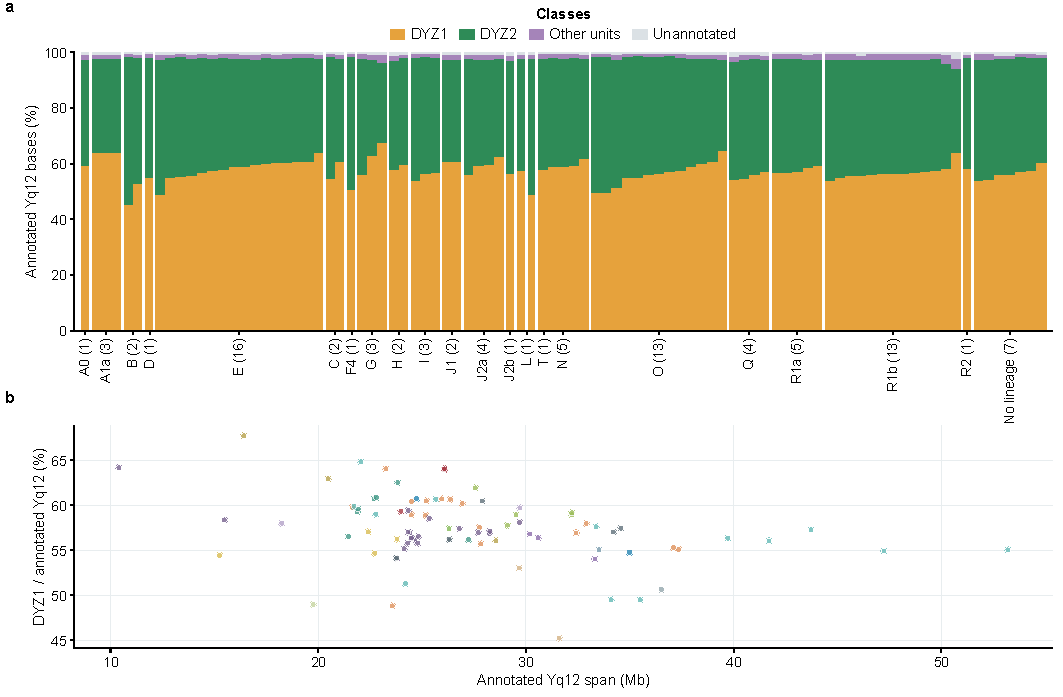
\includegraphics{figures/ed/ed2_yq12_composition.pdf}}
\caption{\textbf{Individual composition of complete Yq12 assembly references.} \textbf{a}, Per-individual composition of all 91 complete reference arrays, grouped by Y clade and sorted by DYZ1 fraction within each clade. Counts below groups give the number of references. The final seven references lack matching lineage metadata. DYZ1, DYZ2, other units (DYZ18, 3.1 kb and 2.7 kb) and residual unannotated bases sum to the annotated Yq12 span. \textbf{b}, DYZ1 fraction against annotated Yq12 span in the same 91 references. Colours denote broad Y lineages as in Supplementary Fig.~\ref{fig:map}. Grey marks references without lineage metadata. The plot is descriptive and both axes use the same span. These are assembly annotations. The read-based population estimates are shown separately in Extended Data Fig.~\ref{fig:s-population}.}\label{fig:yq12-composition}
\end{figure}
\endgroup

\begingroup
\renewcommand{\figurename}{Extended Data Fig.}\renewcommand{\thefigure}{3}
\begin{figure}[p]
\centering
\makebox[\textwidth][c]{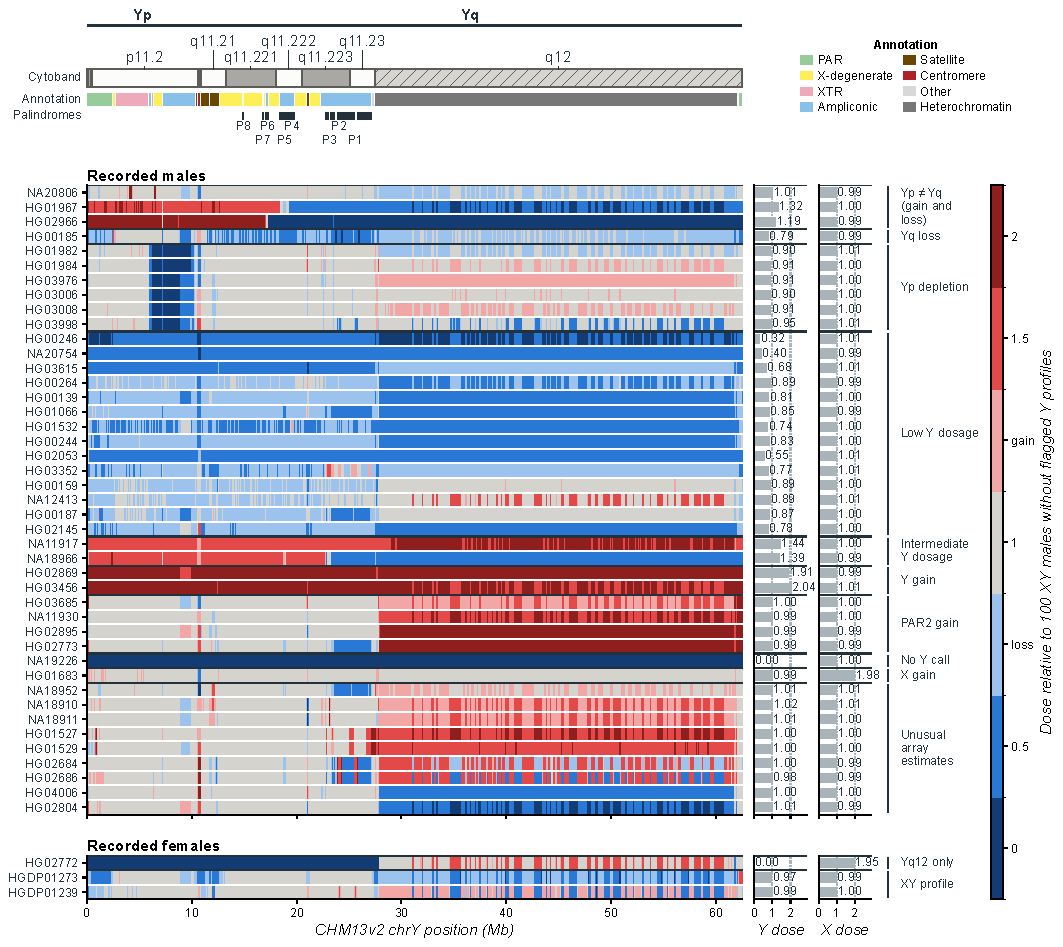
\includegraphics{figures/ed/ed3_chrY_unusual_males.pdf}}
\caption{\textbf{chrY profiles of 1000 Genomes males with an unusual Y state or array estimate.} Each row is one male and each column one of the 625 windows of 100 kb of CHM13v2 chrY. Colours give, in seven steps, the median dose of the chrY 31-mers that occur on no other CHM13 sequence, relative to the median of 100 XY males with Y state normal. In PAR1 and PAR2 the Y dose is twice the dose of the 31-mers shared by chrX and chrY minus the X dose. Top: arms, cytobands, sequence classes \cite{Rhie2023} and palindromes. Right: Y dosage from the single-copy Y ruler and X dosage from 31-mers found only on chrX. Groups follow the Y state rules, and parents and offspring that are both shown are drawn next to each other (HG01982 and HG01984, HG03006 and HG03008, HG02684 and HG02686 of H3b2a, NA18910 and NA18911, HG01527 and HG01529). HG02966 is a parent without the change of its offspring. PAR2 doses in independent data: HG03685 1.58 in nanopore reads (Yq12 and PAR2 on 15p), NA11930 1.43--1.51 in three libraries, HG02895 1.45 and 1.47 in two nanopore runs, HG02773 1.50 in a Polaris library. NA19226 has lost the Y and its offspring is XY. Unusual array estimates: HG02804 (DYZ2), HG04006 and NA18952 (DYZ3), NA18910 and NA18911 (DYZ19), HG01527 and HG01529 (DYZ18S). In the centromere, DYZ19 and Yq12 the value is the array amount relative to the median male, not a chromosome copy number.}\label{fig:chrY-unusual}
\end{figure}
\endgroup

\begingroup
\renewcommand{\figurename}{Extended Data Fig.}\renewcommand{\thefigure}{4}
\begin{figure}[p]
\centering
\makebox[\textwidth][c]{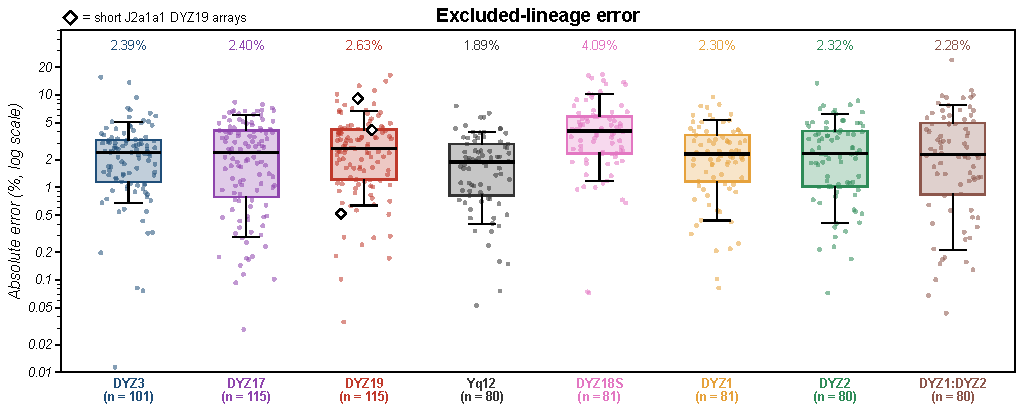
\includegraphics{figures/ed/ed4_lineage_validation.pdf}}
\caption{\textbf{Exclusion of entire Y lineages.} Each point is the single absolute percentage error of one individual when its entire lineage is excluded from training, pooling all 18 excluded-lineage tests. Training also excludes any recorded family shared with test individuals. Squares give the median of the per-individual mean errors of the random cross-validation (Fig.~\ref{fig:method}b) for comparison. Boxes span the 25th--75th percentiles, central lines mark medians and whiskers end at the 10th and 90th percentiles. All individual points are shown, and labels identify the three largest errors per target. Axes are linear through 5\% and logarithmic above.}\label{fig:lineage-validation}
\end{figure}
\endgroup

\begingroup
\renewcommand{\figurename}{Extended Data Fig.}\renewcommand{\thefigure}{5}
\begin{figure}[tbp]
\centering
\makebox[\textwidth][c]{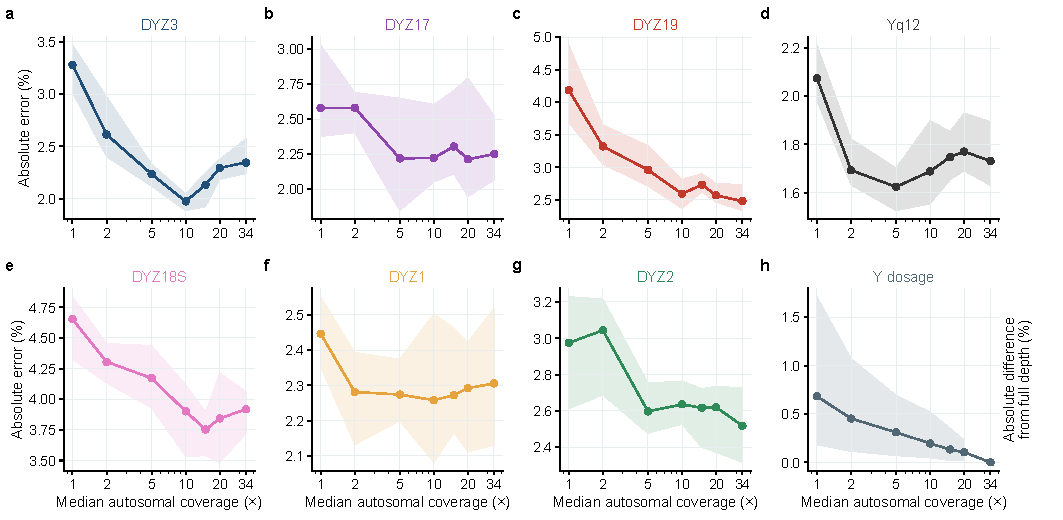
\includegraphics{figures/ed/ed5_depth.pdf}}
\caption{\textbf{Depth sensitivity of all \vsette{seven} targets.} Test reads are thinned to \vsette{20, 15, 10, 5, 2 and 1$\times$ of base coverage and shown with full depth (34.1$\times$)}, while training reads retain full depth. Panels: a DYZ3, b DYZ17, c DYZ19, d Yq12, e DYZ18S, f DYZ1, g DYZ2, h Y dosage. The x-axis gives median autosomal \vsette{base coverage}. Points show the mean of ten grouped-CV repeat-specific median absolute percentage errors, with shading showing their range. These ranges are not confidence intervals. Evaluated counts are \vsette{101 for DYZ3, 115 for DYZ19 and DYZ17, 80 for Yq12 and DYZ2, and 81 for DYZ1 and DYZ18S}. Downsampling reuses the same individuals, and its full-depth baseline matches the ten repeats in Table~\ref{tab:accuracy}. \textbf{h}, Y dosage of the same 119 thinned males, as the median absolute difference from its full-depth value (0 at full depth by definition), with shading from the 10th to the 90th percentile (one thinning per male, with the chr2 window used in training as denominator).}\label{fig:s-depth}
\end{figure}
\endgroup

\begingroup
\renewcommand{\figurename}{Extended Data Fig.}\renewcommand{\thefigure}{6}
\begin{figure}[p]
\centering
\makebox[\textwidth][c]{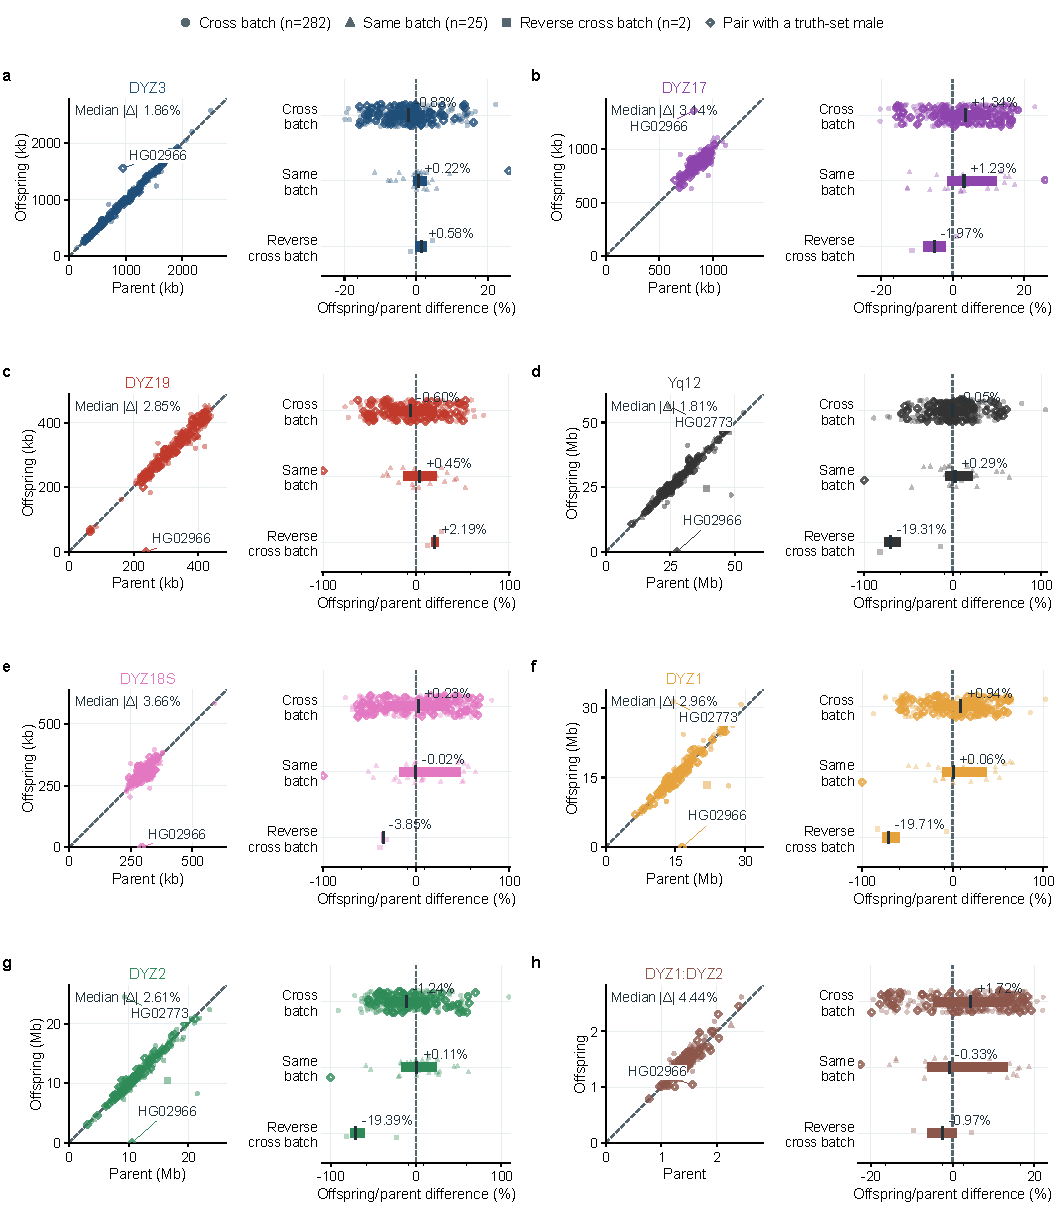
\includegraphics{figures/ed/ed6_pedigrees.pdf}}
\caption{\textbf{Parent--offspring concordance for every satellite target and the DYZ1:DYZ2 length ratio.} \textbf{a--\vsette{h}}, All 309 pairs with complete estimates for the \vsette{seven} targets and the derived ratio (a DYZ3, b DYZ17, c DYZ19, d Yq12, e DYZ18S, f DYZ1, g DYZ2, h DYZ1:DYZ2). Each letter covers the parent-against-offspring plot (left, diagonals mark equality, axes have matching limits) and the signed offspring/parent differences by batch contrast (right, bars: interquartile ranges, ticks: medians, axes linear within $\pm5\%$ and logarithmic outside). Colours match Fig.~\ref{fig:method}b. Shapes distinguish the 282 cross-batch pairs (parent in the original 2,504 samples, offspring in the 698 added in 2020, circles), 25 same-batch pairs (triangles) and two reverse cross-batch pairs (squares). Open diamonds mark the 78 pairs that involve a truth-set male (68 with a calibration male). Annotations give median absolute offspring/parent differences, and labels identify the offspring of the pair with the largest absolute percentage difference and HG02966 when its difference exceeds 20\%, each only above 10\%. All complete profiles, including arm-imbalanced or Yp-depleted profiles, remain visible. No dosage cutoff or batch correction is applied. Targets use their indicated length units, and the ratio is dimensionless. Pedigree pairs can share relatives and are not independent observations.}\label{fig:all-pedigrees}
\end{figure}
\endgroup

\begingroup
\renewcommand{\figurename}{Extended Data Fig.}\renewcommand{\thefigure}{7}
\begin{figure}[tbp]
\centering
\makebox[\textwidth][c]{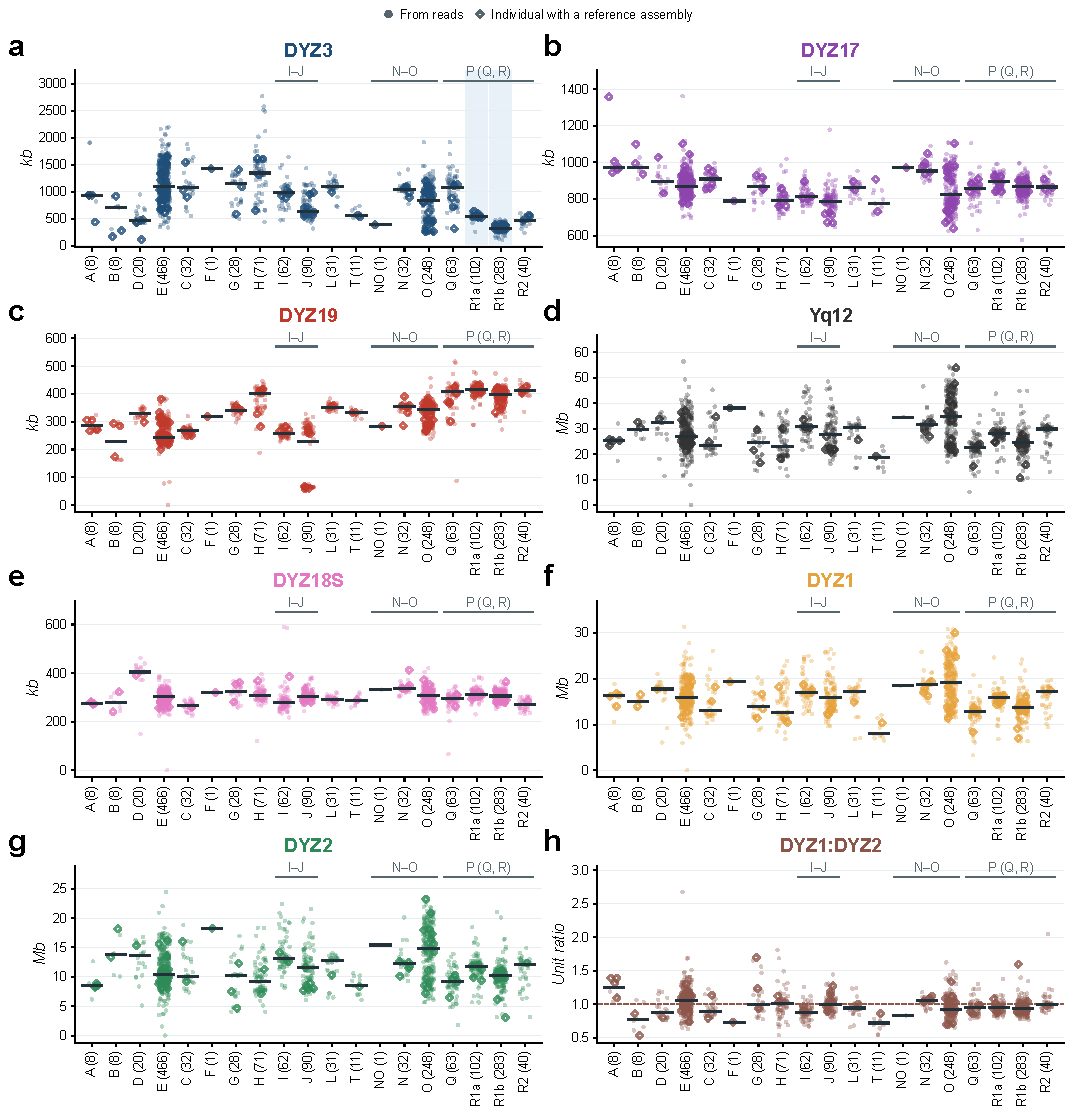
\includegraphics{figures/ed/ed7_population.pdf}}
\caption{\textbf{\vsette{Seven} satellite measurements across the analysed population.} \textbf{a--\vsette{g}}, Estimated lengths by broad Y lineage for all 1,597 males with estimates, retaining rare groups. \textbf{h}, Y dosage relative to the median male (dashed line at 1). Males per lineage: E 466, R1b 283, O 248, R1a 102, J 90, H 71, Q 63, I 62, R 40, C 32, N 32, L 31, G 28, D 20, T 11, A 8, B 8, F 1, NO 1. Horizontal lines show medians. Open diamonds: males whose assembled array of that class is in the truth set. Medians exclude males with arm-imbalanced or Yp-depleted profiles (Extended Data Fig.~\ref{fig:chrY-unusual}). Reference estimates can be in-sample. \vsette{Yq12 is the sum of DYZ1, DYZ2 and the rest of Yq12.} Uneven sampling and family dependence limit population-frequency interpretation.}\label{fig:s-population}
\end{figure}
\endgroup

\begingroup
\renewcommand{\figurename}{Extended Data Fig.}\renewcommand{\thefigure}{8}
\begin{figure}[tbp]
\centering
\makebox[\textwidth][c]{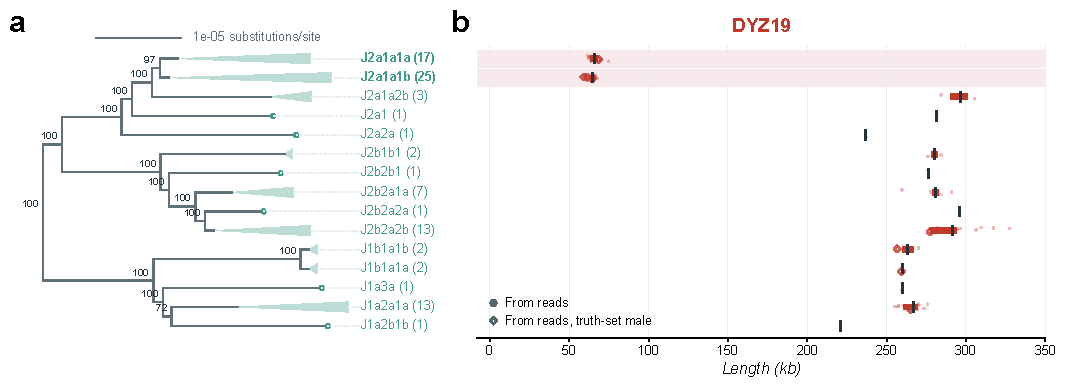
\includegraphics{figures/ed/ed8_J_DYZ19.pdf}}
\caption{\textbf{DYZ19 estimates aligned to the SNP tree of all 90 sampled J chromosomes.} \textbf{a}, Pruned tree retaining branch lengths (scale bar in substitutions per site). Tips give sample identifiers and abbreviated ISOGG 2019 calls. \textbf{b}, Read-based DYZ19 estimates, with J2a1a1 calls in pink and other J calls in purple. Open diamonds mark truth-set males. The short-state groups have distinct J2a1a1a and J2a1a1b calls within a single clade, and J2a1a2 lies outside it. The tree is used descriptively, and the number and timing of state transitions were not inferred.}\label{fig:j-dyz19}
\end{figure}
\endgroup

\begingroup
\renewcommand{\figurename}{Supplementary Fig.}\renewcommand{\thefigure}{1}
\begin{figure}[tbp]
\centering
\makebox[\textwidth][c]{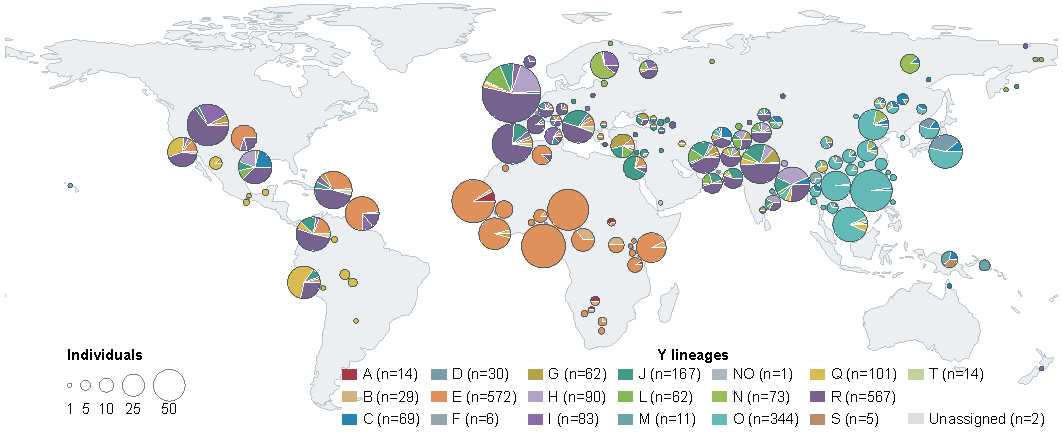
\includegraphics{figures/supp/suppfig1_world_map.pdf}}
\caption{\textbf{Geographic coverage of the cohorts.} 1,597 1kGP individuals with estimates and HGDP/SGDP cohort manifests: 2,302 unique individuals after deduplication. Coordinates are cohort-reported population locations. Pie area scales with sample counts, and sectors and legend counts show paternal Y lineages. Every individual has a lineage call (two from chrY genotypes called for this study). Seven SGDP records reported as female and one additional record without Y signal are excluded (Methods).}\label{fig:map}
\end{figure}
\endgroup

\begingroup
\renewcommand{\figurename}{Supplementary Fig.}\renewcommand{\thefigure}{2}
\begin{figure}[tbp]
\centering
\makebox[\textwidth][c]{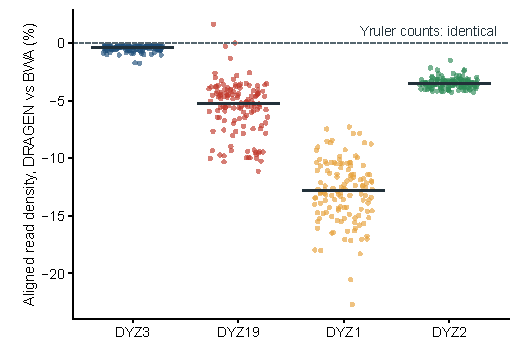
\includegraphics{figures/supp/suppfig2_aligner_depth.pdf}}
\caption{\textbf{Aligned read density depends on the aligner.} The same reads of 130 males, aligned with BWA and with DRAGEN 3.7.6. Each point is one male and shows the change in read density in the GRCh38 array block relative to chrY:14.5--15.5 Mb. Bars show medians. The dashed line marks no change, as obtained for the Yruler counts.}\label{fig:aligner}
\end{figure}
\endgroup


\clearpage



\backmatter

\bmhead{Funding}
This work was made possible, in part, through the generous philanthropic support of the Robert \& Lynda Carter Altman Family Foundation.

\bmhead{Acknowledgements}
We thank the Human Pangenome Reference Consortium and the Human Genome Structural Variation Consortium for the assemblies and reads that made this work possible, and the 1000 Genomes Project, HGDP and SGDP for their public sequencing data.

\section*{Declarations}

\bmhead{Authors' contributions}
A.O.-V. contributed to study validation and comparison analyses, analyzed the data, made the figures and wrote the manuscript. A.G. conceived and designed the study, implemented the method, generated the estimates, performed validations, analyzed the data, made the figures and wrote the manuscript.

\bmhead{Competing interests}
The authors declare no competing interests.

\bmhead{Data availability}
We used public 1000 Genomes sequencing data \cite{ByrskaBishop2022}, HGDP and SGDP sequencing data \cite{Bergstrom2020,Mallick2016}, Y chromosome assemblies \cite{Hallast2026}, HPRC release 2 assemblies and nanopore reads \cite{HPRCRelease2} and pedigree sequencing resources \cite{Porubsky2025}. Public KING reports and corrected sample metadata are available from \url{https://www.cog-genomics.org/plink/2.0/resources}. Independent libraries are in BioProjects PRJNA686136 (low-pass libraries of NA11930 and NA12342), PRJNA909799 (Aviti and NovaSeq libraries of NA11930), PRJEB25009 (Polaris library of HG02773) and PRJEB20654 (Polaris library of HG02771). Nanopore runs are in PRJEB89727 and PRJEB112147 (HG01967, HG02771 and HG02895) and in the 1000 Genomes nanopore data \cite{Gustafson2024} (HG03685 and five control males). Study data (per-sample satellite estimates, reference-array annotations, model parameters, cross-validation predictions, the SNP tree, relatedness tables and geographic metadata) are at \url{https://github.com/AndreaGuarracino/yruler-paper}.
The DYZ1 depth values of San Roman et al.\ are their Table S6A \cite{SanRoman2024}, \url{https://doi.org/10.1016/j.xgen.2023.100462}.
This study generated no new sequencing data. The per-sample estimates, validation predictions and all tables behind the figures are in the analysis repository.

\bmhead{Code availability}
The Yruler repository is \url{https://github.com/guarracinolab/yruler}, under the MIT licence. The analysis code that generates the figures and tables from per-sample estimates, validation predictions and source metadata is at \url{https://github.com/AndreaGuarracino/yruler-paper}, with the scripts that build the model from assemblies and reads in its \texttt{scripts/pipeline} folder.

\bibliography{refs}

\end{document}
